\setcounter{section}{2}

\section{Мінімізація детермінованих скінчених \texorpdfstring{\\}{} автоматів}

\subsection{Мінімізація детермінованих скінчених \texorpdfstring{\\}{} автоматів}

В подальшому при програмуванні скінчених автоматів важливо мати справу з так званими  ``мінімальними автоматами''. \textit{Мінімальним} для даного скінченого автомата називається еквівалентний йому автомат з мінімальною кількістю станів. \medskip

Нагадаємо, що два автомати називаються \textit{еквівалентними} якщо вони розпізнають одну мову. \medskip

Те, що скінчені автомати можна мінімізувати покажемо на наступному прикладі:
\begin{figure}[H]
	\centering
	\section*{Заняття 4: Інтегровані типи диференціальних рівнянь 1-го порядку, розв'язані відносно похідної. Однорідні рівняння та зведені до них. Лінійні рівняння}

\subsection*{Аудиторні задачі}

\begin{problem}
	$\left( y + \sqrt{x^2 + y^2} \right) \cdot \diff x - x \cdot \diff y = 0$.
\end{problem}

\begin{problem}
	$2 x y \cdot \diff x + (y^2 - x^2) \cdot \diff y = 0$.  $M(1,1)$.
\end{problem}

\begin{problem}
	$(2 x + 3 y) \cdot \diff x + (x + 2 y) \cdot \diff y = 0$.
\end{problem}

\begin{problem}
	$x \cdot y' - x \cdot \cos (y / x) - y = 0$.
\end{problem}

\begin{problem}
	$(y^3 + 2 x^2 y) \cdot \diff x - (2 x^3 + 2 x y^2) \cdot \diff y = 0$.
\end{problem}

\begin{problem}
	$(6 x + y - 1) \cdot \diff x + (4 x + y - 2) \cdot \diff y = 0$.
\end{problem}

\begin{problem}
	$(x + y + 1) \cdot \diff x + (2 x + 2 y - 1) \cdot \diff y = 0$.
\end{problem}

\begin{problem}
	$y \cdot (x^2 \cdot y^2 + 1) \cdot \diff x + (x^2 \cdot y^2 - 1) \cdot x \cdot \diff y = 0$.
\end{problem}

\begin{problem}
	$x \cdot y \cdot \diff x + (y^4 - x^2) \cdot \diff y = 0$.
\end{problem}

\begin{problem}
	$\diff y / \diff x - y = 2 x - x^2$.
\end{problem}

\begin{problem}
	$\diff y / \diff x + y \cdot \cos (x) = \sin (x) \cdot \cos (x)$.
\end{problem}

\begin{problem}
	$y' \cdot (x + \cot (y)) = 1$.
\end{problem}

\subsection*{Домашнє завдання}

\begin{problem}
	$x \cdot y' = y \cdot (1 + \ln (y) - \ln (x))$.
\end{problem}

\begin{problem}
	$x \cdot \diff y - \left( \sqrt{x^2 + y^2} + y \right) \cdot \diff x = 0$.
\end{problem}

\begin{problem}
	$\left( x y \cdot e^{x / y} + y^2 \right) \cdot \diff x - x^2 \dot e^{x / y} \cdot \diff y = 0$.
\end{problem}

\begin{problem}
	$(6 x y + 5 y^2) \cdot \diff x + (3 x^2 + 10 x y - y^2) \cdot \diff y = 0$.
\end{problem}

\begin{problem}
	$(x^3 + 3 x y^2) \cdot (2 y^3 + 3 x^2 y) \cdot \diff y = 0$.
\end{problem}

\begin{problem}
	$(x - 2) \cdot \diff x + (y - 2 x + 1) \cdot \diff y = 0$.
\end{problem}

\begin{problem}
	$(x + 2 y - 1) \cdot \diff x + (2 x + 4 y + 3) \cdot \diff y = 0$.
\end{problem}

\begin{problem}
	$y^3 \cdot \diff x + 2 \cdot (x^2 - x y^2) \cdot \diff y = 0$.
\end{problem}

\begin{problem}
	$(x y^2 - y) \cdot \diff x - (x^3 y^2 - 3 x^2 y + 3 x) \cdot \diff y = 0$.
\end{problem}

\begin{problem}
	$\diff y / \diff x - y = x - 1$.  $M(0,1)$.
\end{problem}

\begin{problem}
	$y' + y = \sin (x) + \cos (x)$.
\end{problem}

\begin{problem}
	$y' \cdot (x + \ln (y)) = 1$.
\end{problem}

\end{figure}

Навіть при поверхневому аналізі діаграми переходів наведеного скінченого автомата видно, що вершини $q_3$, $q_4$ та $q_5$ є ``зайвими'', тобто при їх вилученні новий автомат буде еквівалентний початковому. З наведеного вище прикладу видно, що для отриманого детермінованого скінченого автомата можна запропонувати еквівалентний йому автомат з меншою кількістю станів, тобто мінімізувати скінчений автомат. Очевидно що серед зайвих станів цього автомата є недосяжні та тупикові стани.

\subsubsection{Недосяжні стани}

Стан $q$ скінченого автомата $M$ називається \textit{недосяжним}, якщо на діаграмі переходів скінченого автомата не існує шляху з $q_0$ в $q$. \medskip

\textbf{Алгоритм [пошуку недосяжних станів].} Спочатку спробуємо побудувати множину досяжних станів. Якщо $Q_m$ --- множина досяжних станів скінченого автомата $M$, то $Q \setminus Q_m$ --- множина недосяжних станів. Побудуємо послідовність множин $Q_0, Q_1, Q_2, \ldots$ таким чином, що:
\begin{enumerate}
	\item $Q_0 = \{q_0\}$.
	\item $Q_i = Q_{i-1} \cup \left\{ q \mid \exists a \in \Sigma, q_j \in Q_{i - 1}: q \in \delta(q_j, a) \right\}$.
	\item $Q_m = Q_{m+1} = \ldots$.
\end{enumerate}

Справді, очевидно, що кількість кроків скінчена, тому що послідовність $Q_i$ монотонна $\left(Q_0 \subseteq Q_1 \subseteq Q_2 \subseteq \ldots\right)$ та обмежена зверху: $Q_m \subseteq Q$. \medskip

Тоді $Q_m$ --- множина досяжних станів скінченого автомата, а $Q\setminus Q_m$ --- множина недосяжних станів. \medskip

Вилучимо з діаграми переходів скінченого автомата $M$ недосяжні вершини:
\begin{figure}[H]
	\centering
	 % cd ..\..\Users\NikitaSkybytskyi\Desktop\c3s1\complex-analysis
\documentclass[a4paper, 12pt]{article}
\usepackage[utf8]{inputenc}
\usepackage[english, ukrainian]{babel}

\usepackage{amsmath, amssymb}
\usepackage{multicol}
\usepackage{graphicx}
\usepackage{float}
\usepackage{multicol}

\usepackage{amsthm}
\newtheorem{theorem}{Теорема}[subsection]
\newtheorem*{theorem*}{Теорема}
\newtheorem{lemma}{Лема}[subsection]
\newtheorem*{lemma*}{Лема}
\newtheorem*{remark*}{Зауваження}
\theoremstyle{definition}
\newtheorem*{definition}{Визначення}
\newtheorem{problem}{Задача}[section]
\newtheorem*{solution}{Розв'язок}
\newtheorem{example}{Приклад}
\newtheorem*{example*}{Приклад}
\newtheorem*{hint}{Вказівка}

\newcommand{\Max}{\displaystyle\max\limits}
\newcommand{\Sum}{\displaystyle\sum\limits}
\newcommand{\Int}{\displaystyle\int\limits}
\newcommand{\Lim}{\displaystyle\lim\limits}

\newcommand{\RR}{\mathbb{R}}
\newcommand{\ZZ}{\mathbb{Z}}

\newcommand*\diff{\mathop{}\!\mathrm{d}}
\newcommand*\Diff[1]{\mathop{}\!\mathrm{d^#1}}

\DeclareMathOperator{\Real}{Re}
\DeclareMathOperator{\Imag}{Im}

\DeclareMathOperator{\Arg}{Arg}

\DeclareMathOperator{\Ln}{Ln}

\DeclareMathOperator{\Arctan}{Arctan}
\DeclareMathOperator{\Arcsin}{Arcsin}
\DeclareMathOperator{\Arccos}{Arccos}
\DeclareMathOperator{\Arccosh}{Arccosh}
\DeclareMathOperator{\Arctanh}{Arctanh}

\DeclareMathOperator{\arcsinh}{arcsinh}
\DeclareMathOperator{\arccosh}{arccosh}
\DeclareMathOperator{\arctanh}{arctanh}
\DeclareMathOperator{\arccoth}{arccoth}

\newcommand{\varLimsup}{\varlimsup\limits}

\makeatletter
\newcommand\xLeftrightarrow[2][]{%
  \ext@arrow 9999{\longLeftrightarrowfill@}{#1}{#2}}
\newcommand\longLeftrightarrowfill@{%
  \arrowfill@\Leftarrow\relbar\Rightarrow}
\makeatother

\renewcommand{\epsilon}{\varepsilon}
\renewcommand{\phi}{\varphi}

\allowdisplaybreaks
\setlength\parindent{0pt}
\numberwithin{equation}{subsection}

\usepackage{xcolor}
\usepackage{hyperref}
\hypersetup{unicode=true,colorlinks=true,linktoc=all,linkcolor=red}

\numberwithin{equation}{section}% reset equation counter for sections
\numberwithin{equation}{subsection}
% Omit `.0` in equation numbers for non-existent subsections.
\renewcommand*{\theequation}{%
  \ifnum\value{subsection}=0 %
    \thesection
  \else
    \thesubsection
  \fi
  .\arabic{equation}%
}


 \title{{\Huge МАТЕМАТИЧНА ФІЗИКА}}
 \author{Скибицький Нікіта}
 \date{\today}

 \usepackage{amsthm}
\usepackage[dvipsnames]{xcolor}
\usepackage{thmtools}
\usepackage[framemethod=TikZ]{mdframed}

\theoremstyle{definition}
\mdfdefinestyle{mdbluebox}{%
	roundcorner = 10pt,
	linewidth=1pt,
	skipabove=12pt,
	innerbottommargin=9pt,
	skipbelow=2pt,
	nobreak=true,
	linecolor=blue,
	backgroundcolor=TealBlue!5,
}
\declaretheoremstyle[
	headfont=\sffamily\bfseries\color{MidnightBlue},
	mdframed={style=mdbluebox},
	headpunct={\\[3pt]},
	postheadspace={0pt}
]{thmbluebox}

\mdfdefinestyle{mdredbox}{%
	linewidth=0.5pt,
	skipabove=12pt,
	frametitleaboveskip=5pt,
	frametitlebelowskip=0pt,
	skipbelow=2pt,
	frametitlefont=\bfseries,
	innertopmargin=4pt,
	innerbottommargin=8pt,
	nobreak=true,
	linecolor=RawSienna,
	backgroundcolor=Salmon!5,
}
\declaretheoremstyle[
	headfont=\bfseries\color{RawSienna},
	mdframed={style=mdredbox},
	headpunct={\\[3pt]},
	postheadspace={0pt},
]{thmredbox}

\declaretheorem[%
style=thmbluebox,name=Теорема,numberwithin=section]{theorem}
\declaretheorem[style=thmbluebox,name=Лема,sibling=theorem]{lemma}
\declaretheorem[style=thmbluebox,name=Твердження,sibling=theorem]{proposition}
\declaretheorem[style=thmbluebox,name=Наслідок,sibling=theorem]{corollary}
\declaretheorem[style=thmredbox,name=Приклад,sibling=theorem]{example}

\mdfdefinestyle{mdgreenbox}{%
	skipabove=8pt,
	linewidth=2pt,
	rightline=false,
	leftline=true,
	topline=false,
	bottomline=false,
	linecolor=ForestGreen,
	backgroundcolor=ForestGreen!5,
}
\declaretheoremstyle[
	headfont=\bfseries\sffamily\color{ForestGreen!70!black},
	bodyfont=\normalfont,
	spaceabove=2pt,
	spacebelow=1pt,
	mdframed={style=mdgreenbox},
	headpunct={ --- },
]{thmgreenbox}

\mdfdefinestyle{mdblackbox}{%
	skipabove=8pt,
	linewidth=3pt,
	rightline=false,
	leftline=true,
	topline=false,
	bottomline=false,
	linecolor=black,
	backgroundcolor=RedViolet!5!gray!5,
}
\declaretheoremstyle[
	headfont=\bfseries,
	bodyfont=\normalfont\small,
	spaceabove=0pt,
	spacebelow=0pt,
	mdframed={style=mdblackbox}
]{thmblackbox}

% \theoremstyle{theorem}
\declaretheorem[name=Запитання,sibling=theorem,style=thmblackbox]{ques}
\declaretheorem[name=Вправа,sibling=theorem,style=thmblackbox]{exercise}
\declaretheorem[name=Зауваження,sibling=theorem,style=thmgreenbox]{remark}

\theoremstyle{definition}
\newtheorem{claim}[theorem]{Твердження}
\newtheorem{definition}[theorem]{Визначення}
\newtheorem{fact}[theorem]{Факт}

\newtheorem{problem}{Задача}[section]
\renewcommand{\theproblem}{\thesection\Alph{problem}}
\newtheorem{sproblem}[problem]{Задача}
\newtheorem{dproblem}[problem]{Задача}
\renewcommand{\thesproblem}{\theproblem$^{\star}$}
\renewcommand{\thedproblem}{\theproblem$^{\dagger}$}
\newcommand{\listhack}{$\empty$\vspace{-2em}} 

 \begin{document}

 \tableofcontents

% \section{Аналіз похибок заокруглення}

\subsection{Види похибок}

Нехай необхідно розв’язати рівняння
\begin{equation}
	\label{eq:1.1}
	Au = f.
\end{equation}
За рахунок неточно заданих вхідних даних насправді ми маємо рівняння
\begin{equation}
	\label{eq:1.2}
	\tilde A \tilde u = \tilde f.
\end{equation}
Назвемо $\delta_1 = u - \tilde u$ -- \textit{неусувною похибкою}. \\

Застосування методу розв‘язання \eqref{eq:1.2} приводить до рівняння
\begin{equation}
	\label{eq:1.3}
	\tilde A_h \tilde u_h = \tilde f_h,
\end{equation}
де $h > 0$ -- малий параметр. Назвемо $\delta_2 \tilde u - \tilde u_h$ -- \textit{похибкою методу}. \\

Реалізація методу на ЕОМ приводить до рівняння
\begin{equation}
	\label{eq:1.4}
	\tilde A_h^* \tilde u_h^* = \tilde f_h^*.
\end{equation}
Назвемо $\delta_3 = \tilde u_h^* - \tilde u_h$ -- \textit{похибкою заокруглення}. \\

Тоді \textit{повна похибка} $\delta = u - \tilde u_h^* = \delta_1 + \delta_2 + \delta_3$. \\

\begin{definition}
	Кажуть, що задача \eqref{eq:1.1} \textit{коректна}, якщо
	\begin{enumerate}
		\item $\forall f \in F$ $\exists! u \in U$;
		\item задача \eqref{eq:1.1} \textit{стійка}, тобто
		\begin{equation}
			\label{eq:1.5}
			\forall \epsilon > 0 \quad \exists \delta > 0: \|A-\tilde A\| < \delta, \|f-\tilde f\| < \delta \Rightarrow \|u - \tilde u\| < \epsilon.
		\end{equation}
	\end{enumerate}
\end{definition}

Якщо задача \eqref{eq:1.1} \textit{некоректна}, то або розв‘язок її не існує, або він неєдиний, або він нестійкий, тобто 
\begin{equation}
	\label{eq:1.6}
	\exists \epsilon > 0: \forall \delta > 0: \exists A, f: \| A - \tilde A\|<\delta, \|f-\tilde f\| < \delta, \|u-\tilde u\| > \epsilon.
\end{equation}

\textit{Абсолютна похибка} $\Delta (x^*) \ge \max_x |x - x^*|$. \\

\textit{Відносна похибка} $\delta (x^*) \ge \max_x \Delta (x^*) / |x^*|$. \\

\textit{Значущими цифрами} називаються всі цифри, починаючи з першої ненульової зліва. \\

\textit{Вірна цифра} -- це значуща, якщо абсолютна похибка за рахунок відкидання всіх молодших розрядів не перевищує одиниці розряду цієї цифри. Тобто, якщо 
\begin{equation}
	\label{eq:1.7}
	x^* = \overline{\alpha_n \ldots \alpha_0.\alpha_{-1}\ldots\alpha_{-p}\ldots},
\end{equation}
то $\alpha_{-p}$ -- вірна, якщо $\Delta (x^*) \le 10^{-p}$. \\

Інколи $\Delta (x^*) \le w \cdot 10^{-p}$, $1/2 \le w < 1$, наприклад, $w = 0.55$.

\subsection{Підрахунок похибок в ЕОМ}

Підрахуємо відносну похибку заокруглення числа $x$ на ЕОМ з плаваючою комою. В $\beta$-ічній системі числення число представляється у вигляді
\begin{equation}
	\label{eq:1.8}
	x = \pm (\alpha_1 \beta^{-1} + \alpha_2 \beta^{-2} + \ldots + \alpha_t \beta^{-t} + \ldots) \beta^p,
\end{equation}
де $0 \le \alpha_k < \beta$, $\alpha_1 \ne 0$, $k = 1,2,\ldots$ \\

Якщо в ЕОМ $t$ розрядів, то при відкиданні молодших розрядів ми оперуємо з наближеним значенням 
\begin{equation}
	\label{eq:1.9}
	x^* = \pm (\alpha_1 \beta^{-1} + \alpha_2 \beta^{-2} + \ldots + \alpha_t \beta^{-t}) \beta^p,
\end{equation}
і відповідно похибка заокруглення 
\begin{equation}
	\label{eq:1.9_1}
	x - x^* = \pm \beta^p (\alpha_{t+1} \beta^{-t-1} + \ldots)
\end{equation}
Тоді її можна оцінити так
\begin{multline}
	\label{eq:1.10}
	|x - x^*| \le \beta^{p-t-1} \cdot (\beta-1) \cdot (1 + \beta^{-1}+\ldots)\le\\
	\le \beta^{p-t-1} \cdot (\beta-1) \cdot \dfrac{1}{1-\beta^{-1}}=\beta^{p-t}.
\end{multline}

Якщо в представлені \eqref{eq:1.8} взяти $\alpha_1 = 1$, то $|x| \ge \beta^p \cdot \beta^{-1}$. Звідси остаточно 
\begin{equation}
	\label{eq:1.11}
	\delta (x^*) \le \dfrac{\beta^{p-t}}{\beta^{p-1}}=\beta^{1-t}.
\end{equation}

При більш точних способах заокруглення можна отримати оцінку $\delta (x^*) \le \beta^{1-t} / 2 = \epsilon$. Число $\epsilon$ називається ``машинним іпсилон''. Наприклад, для $\beta = 2$, $t = 24$, $\epsilon = 2^{-24} \approx 10^{-7}$.

\subsection{Підрахунок похибок обчислення значення функції}

Нехай задана функція 
\begin{equation}
	\label{eq:1.11_1}
	y = f(x_1, \ldots, x_n) \in C^1(\Omega)
\end{equation}
Необхідно обчислити її значення при наближеному значенні аргументів 
\begin{equation}
	\label{eq:1.11_2}
	\vec x^* = (x_1^*, \ldots, x_n^*),
\end{equation}
де $|x_i - x_i^*| \le \Delta (x_i^*)$ та оцінити похибку обчислення значення функції
\begin{equation}
	\label{eq:1.11_3}
	y^* = f(x_1^*, \ldots, x_n^*).
\end{equation}

Маємо 
\begin{equation}
	\label{eq:1.12}
	|y-y^*| = |f\left(\vec x\right) - f\left(\vec x^*\right)| = \left| \Sum_{i=1}^n \dfrac{\partial f}{\partial x_i} \left(\vec \xi\right) (x_i - x_i^*) \right| \le \Sum_{i=1}^n B_i \cdot \Delta (x_i^*), 
\end{equation}
де 
\begin{equation}
	\label{eq:1.13}
	B_i = \Max_{\vec x \in U} \left| \dfrac{\partial f}{\partial x_i}\left(\vec x\right) \right|.
\end{equation}

Тут 
\begin{equation}
	\label{eq:1.14}
	U = \left\{ \vec x = (x_1, \ldots, x_n): |x_i - x_i^*| \le \Delta (x_i^*)\right\} \in \Omega, \quad i=\overline{1,n}.
\end{equation}
Отже
\begin{equation}
	\label{eq:1.15}
	\Delta (y^*) = |y - y^*| \prec \Sum_{i=1}^n n_i \cdot \Delta (x_i^*),
\end{equation}
з точністю до величин першого порядку малості по
\begin{equation}
	\label{eq:1.15_1}
	\Delta (x^*) = \Max_{i=\overline{1,n}} \Delta (x_i^*),
\end{equation}
де
\begin{equation}
	\label{eq:1.16}
	b_i = \left| \dfrac{\partial f}{\partial x_i}\left(\vec x^*\right) \right|
\end{equation}
та ``$\prec$'' означає приблизно менше. \\

\subsubsection{Похибки арифметичних операцій}

\begin{enumerate}
	\item Сума: $y = x_1 + x_2$, $x_1, x_2 > 0$, 
	\begin{equation}
		\label{eq:1.17}
		\begin{aligned}
		\Delta (y^*) &\le \Delta (x_1^*) + \Delta (x_2^*), \\ 
		\delta (y^*) &\le \dfrac{\Delta (x_1^*) + \Delta (x_2^*)}{x_1^* + x_2^*} \le \max\{\delta (x_1^*), \delta (x_2^*)\}.
		\end{aligned}
	\end{equation}
	
	\item Різниця: $y = x_1 - x_2$, $x_1 > x_2 > 0$,
	\begin{equation}
		\label{eq:1.18}
		\begin{aligned}
		\Delta (y^*) &\le \Delta (x_1^*) + \Delta (x_2^*), \\
		\delta (y^*) &\le \dfrac{x_2^* \delta (x_1^*) + (x_1^*) \delta (x_2^*)}{x_1^* - x_2^*}.
		\end{aligned}
	\end{equation}
	
	При близьких $x_1^*$, $x_2^*$ зростає відносна похибка (за рахунок втрати вірних цифр).

	\item Добуток: $y = x_1 \cdot x_2$, $x_1, x_2 > 0$,
	\begin{equation}
		\label{eq:1.19}
		\begin{aligned}
		\Delta (y^*) &\prec x_2^* \Delta (x_1^*) + x_1^* \Delta (x_2^*), \\
		\delta (y^*) &\le \delta (x_1^*) + \delta (x_2^*).
		\end{aligned}
	\end{equation}

	\item Частка: $y = \dfrac{x_1}{x_2}$, $x_1, x_2 > 0$,
	\begin{equation}
		\label{eq:1.20}
		\begin{aligned}
		\Delta (y^*) &\prec \dfrac{x_2^* \Delta (x_1^*) + x_1^* \Delta (x_2^*)}{(x_2^*)^2}, \\
		\delta (y^*) &\le \delta (x_1^*) + \delta (x_2^*).
		\end{aligned}
	\end{equation}

	При малих $x_2^*$ зростає абсолютна похибка (за рахунок зростання результату ділення). 
\end{enumerate}

\subsection{Обернена задача аналізу позибок}

Нагадаємо, що \textit{пряма задача} аналізу похибок полягає у обчисленні $\Delta (y^*), \delta (y^*)$ по заданих $\Delta (x_i^*)$, $i = \overline{1, n}$. \\

\textit{Обернена задача} полягає у знаходженні $\Delta (x_i^*)$, $i = \overline{1, n}$ по заданих $\Delta (y^*)$, $\delta (y^*)$. Якщо $n > 1$, маємо одну умову 
\begin{equation}
	\label{eq:1.21}
	\Sum_{i=1}^n b_i \Delta (x_i^*) < \epsilon
\end{equation}
для багатьох невідомих $\Delta (x_i^*)$. Вибирають їх із однієї з умов 
\begin{equation}
	\label{eq:1.22}
	b_i \Delta (x_i^*) < \dfrac{\epsilon}{n},
\end{equation}
або
\begin{equation}
	\label{eq:1.23}
	\Delta (x_i^*) < \dfrac{\epsilon}{\Sum_{i=1}^n b_i}.
\end{equation}
% \section{Нелінійні рівняння}

\textit{Постановка задачі}. Нехай маємо рівняння $f(x) = 0$, $\overline{x}$ -- його розв’язок, тобто $f (\overline{x}) \equiv 0$. \\

Задача розв‘язання цього рівняння розпадається на етапи:
\begin{enumerate}
	\item Існування та кількість коренів.
	\item Відділення коренів, тобто розбиття числової вісі на інтервали, де знаходиться один корінь.
	\item Обчислення кореня із заданою точністю $\epsilon$.
\end{enumerate}

Для розв'язання перших двох задач використовуються методи математичного аналізу та алгебри, а також графічний метод. Далі розглядаються методи розв'язання третього етапу.

\subsection{Метод ділення навпіл}

Припустимо на $[a, b]$ знаходиться лише один корінь рівняння 
\begin{equation}
	\label{eq:2.1}
	f(x) = 0,
\end{equation}
для $f(x) \in C([a,b])$, який необхідно визначити. Нехай $f(a) \cdot f (b) < 0$. \\

Припустимо, що $f(a) > 0$, $f(b) < 0$. Покладемо $x_1 = \frac{a + b}{2}$ і підрахуємо
$f(x_1)$. Якщо $f_1(x) < 0$, тоді шуканий корінь $x$ знаходиться на інтервалі $(a, x_1)$. Якщо ж $f_1(x) > 0$, то $\overline{x} \in (x_1, b)$, тобто з двох інтервалів $(a, x_1)$ і $(x_1, b)$ вибираємо той, на границях якого функція $f(x)$ має різні знаки, знаходимо точку $x_2$ -- середину вибраного інтервалу, підраховуємо $f(x_2)$ і повторюємо вказаний процес. \\

В результаті отримаємо послідовність інтервалів, що містять шуканий корінь $\overline{x}$, причому довжина кожного послідуючого інтервалу вдвічі менше попереднього. \\

Цей процес продовжується до тих пір, поки довжина отриманого інтервалу $(a_n, b_n)$ не стане меншою за $b_n - a_n < 2 \epsilon$. Тоді $x_{n+1}$, як середина інтервалу $(a_n, b_n)$ пов'язане з $\overline{x}$ нерівністю
\begin{equation}
	\label{eq:2.2}
	|x_n+1 - \overline{x}| < \epsilon.
\end{equation}

Ця умова для деякого $n$ буде виконуватись за теоремою Больцано-Коші. \\

Оскільки
\[ |b_{k + 1} - a_{k + 1} | = \dfrac12 |b_k - a_k|, \]
то
\begin{equation}
	\label{eq:2.3}
	|x_{n+1} - \overline{x}| \le \dfrac{1}{2^{n+1}} (b - a) < \epsilon.
\end{equation}

Звідси отримаємо нерівність для обчислення кількості ітерацій $n$ для виконання умови (\ref{eq:2.2}):
\[ n = n(\epsilon) \ge \left\lfloor \log\left(\dfrac{b-a}{\epsilon}\right) \right\rfloor + 1. \]

Степінь збіжності -- лінійна, тобто геометричної прогресії з знаменником $q = \frac12$. \\

Переваги методу: простота, надійність. Недоліки методу: низька швидкість збіжності; метод не узагальнюється на системи. 

\subsection{Метод простої ітерації}

Спочатку рівняння
\begin{equation}
	\label{eq:2.4}
	f (x) = 0
\end{equation}
замінюється еквівалентним
\begin{equation}
	\label{eq:2.5}
	x = \phi(x)
\end{equation}
Ітераційний процес має вигляді
\begin{equation}
	\label{eq:2.6}
	x_{n+1} = \phi(x_n), \quad n = 0,1,\ldots
\end{equation}

Початкове наближення $x_0$ задається. \\

Для збіжності велике значення має вибір функції $\phi(x)$. Перший спосіб заміни рівняння полягає в відділенні змінної з якогось члена рівняння. Більш продуктивним є перехід від рівняння (\ref{eq:2.4}) до (\ref{eq:2.5}) з функцією $\phi (x) = x + \tau (x) \cdot f (x)$, де $\tau (x)$ -- знакостала функція на тому відрізку, де шукаємо корінь. \\

Кажуть, що ітераційний метод \textit{збігається}, якщо $\Lim_{k\to\infty} x_k = \overline{x}$. \\

Далі $U_r = \{x : |x - a| \le r\}$ відрізок довжини $2r$ з серединою в точці $a$. \\

З'ясуємо умови, при яких збігається метод простої ітерації.

\begin{theorem}
	Якщо $\Max_{x \in U_r} |\phi'(x)| \le q < 1$, то метод простої ітерації збігається і має місце оцінка 
	\begin{equation}
		\label{eq:2.7}
		|x_n - \overline{x}| \le \dfrac{q^n}{1-q}|x_0-x_1| \le \dfrac{q^n}{1-q}(b-a).
	\end{equation}
\end{theorem}

\begin{proof}
	Нехай $x_{k+1}, x_k \in U_r$. Тоді має місце допоміжна нерівність:
	\begin{multline*}
		|x_{k+1} - x_k| = |\phi(x_k) - \phi(x_{k-1})| = |\phi'(\xi_k)(x_k - x_{k-1}) \le (*) \\
		\text{тут }\xi_k = x_k + \theta_k (x_{k+1} - x_k), \quad 0 < \theta_k < 1 \\
		(*) \le |\phi'(\xi_k)| \cdot |x_k - x_{k-1}| \le q |x_k - x_{k-1}| = \ldots = q^k |x_1 - x_0|.
	\end{multline*}
	Використаємо її для доведення теореми:
	\begin{multline}
		\label{eq:2.8}
		|x_{k+p} - x_k| = |x_{k+p} - x_{k+p-1} + \ldots + x_{k+1} - x_k| \le \\
		\le |x_{k+p} - x_{k+p-1}| + \ldots + |x_{k+1} - x_k| \le \\
		\le (q^{k+p-1}+q^{k+p-2}+\ldots+q^k) |x_1 - x_0| = \\
		= \dfrac{q^k - q^{k+p-1}}{1-q}|x_1-x_0| \xrightarrow[k\to\infty]{}0.
	\end{multline}

	Бачимо що $\{x_k\}$ -- фундаментальна послідовність. Значить вона збіжна. При $p\to\infty$ в (\ref{eq:2.8}) отримуємо (\ref{eq:2.7}).
\end{proof}

Визначимо кількість ітерацій для досягнення точності $\epsilon$. З оцінки в теоремі отримаємо \[ |x_n - \overline{x}| \le \dfrac{q^n}{1-q}(b-a) < \epsilon \Rightarrow n(\epsilon) = n \ge \left\lfloor \dfrac{\ln \left(\dfrac{\epsilon (1-q)}{b - a}\right)}{\ln q} \right\rfloor + 1. \]

Практично ітераційний процес зупиняємо при: $|x_n - x_{n-1}| < \epsilon$. Але ця умова не завжди гарантує, що $|x_n - \overline{x}| < \epsilon$.

\begin{remark*}
	Умова збіжності методу може бути замінена на умову Ліпшиця \[|\phi(x) -\phi(y)| \le q \cdot| x - y |,\quad 0 < q < 1.\]
\end{remark*}

Переваги методу: простота; при $q < \frac12$ -- швидше збігається ніж метод ділення навпіл; метод узагальнюється на системи. Недоліки методу: 
\begin{enumerate}
	\item при $q > \frac12$ -- збігається повільніше ніж метод ділення навпіл,
	\item виникають труднощі при зведенні $f (x) = 0$ до $x =\phi (x)$.
\end{enumerate}


\subsection{Метод релаксації}

Якщо в методі простої ітерації для рівняння $x = x +\tau f (x) \equiv\phi (x)$ вибрати $\tau (x) =\tau = \const$, то ітераційний процес приймає вигляд
\begin{equation}
	\label{eq:2.9}
	x_{n+1} = x_n +\tau \cdot f(x_n), \quad n = 0,1,2,\ldots
\end{equation}
$x_0$ -- задано. Метод можна записати у вигляді \[\dfrac{x_{k+1}-x_k}{\tau} = f(x_k), \quad k=0,1,\ldots.\] Оскільки $\phi'(x) =1+\tau\cdot f'(x)$, то метод збігається при умові \[ |\phi'(x)| = |1+\tau \cdot f'(x)| \le q < 1.\]

Нехай $f'(x) < 0$, тоді (\ref{eq:2.7}) запишеться у вигляді: $-q \le 1 +\tau \cdot f'(x) \le q < 1$. Звідси \[\tau \cdot |f'(x_k)| \le 1 + q < 2 \quad \text{і} \quad 0 < \tau < \dfrac{2}{|f'(x)|}. \]

Поставимо задачу знаходження $\tau$, для якого $q = q(\tau) \to \min$. Для того, щоб вибрати оптимальний параметр $\tau$, розглянемо рівняння для похибки $z_k = x_j - \overline{x}$. \\

Підставивши $x_k = x + z_k$ в (\ref{eq:2.9}), отримаємо
\[ z_{k+1} = z_k + \tau \cdot f(\overline{x} + z_k).\]

В припущені $f(x)\in C^{(1)}([a,b])$ з теореми про середнє маємо
\[ f(\overline{x} + z_k) = f(\overline{x}) + z_k \cdot f'(\overline{x} + \theta z_k) = z_k \cdot f'(\overline{x}+\theta z_k) = z_k \cdot f'(\xi_k), \]
\[ z_{k+1} = z_k + \tau \cdot f'(\xi_k) \cdot z_k, \]
\[ |z_{k+1}| \le |1 + \tau \cdot f'(\xi_k)| \cdot |z_k| \le \Max_{\xi_k \in U} |1 + \tau \cdot f'(\xi_k)| \cdot |z_k|, \]
\[ |z_{k+1}| \le \max \{|1-\tau \cdot M_1|, |1-\tau \cdot m_1| \}\cdot |z_k|, \]
\[ m_1 = \Min_{x\in[a,b]} |f'(x)|, \quad M_1 = \Max_{x\in[a,b]} |f'(x)|. \]

Таким чином, задача вибору оптимального параметра зводиться до знаходження $\tau$, для якого функція \[ q(\tau) = \max\{|1-\tau \cdot M_1|,|1-\tau \cdot m_1|\}\]
приймає мінімальне значення: $q(\tau)\to\min$.

\begin{figure}[H]
	\centering
	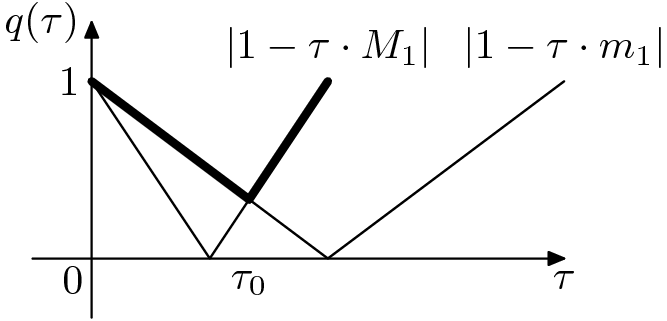
\includegraphics[width=.5\linewidth]{mal-1.png}
\end{figure}

% u:=1cm;
% label.llft(btex $0$ etex, (0,0));
% label.lft(btex $1$ etex, (0,3u/2));
% drawarrow (-u/2,0)--(4u,0);
% drawarrow (0,-u/2)--(0,2u);
% label.lft(btex $q(\tau)$ etex, (0,2u));
% label.bot(btex $\tau$ etex, (4u,0));
% draw (0,3u/2)--(u,0)--(2u,3u/2);
% draw (0,3u/2)--(2u,0)--(4u,3u/2);
% label.top(btex $|1-\tau \cdot M_1|$ etex, (2u,3u/2));
% label.top(btex $|1-\tau \cdot m_1|$ etex, (4u,3u/2));
% draw (4/3u,u/2)--(2u,3u/2) withpen pencircle scaled 2bp;
% draw (0,3u/2)--(4/3u,u/2) withpen pencircle scaled 2bp;
% label.bot(btex $\tau_0$ etex, (4/3u,0));

З графіка видно, що точка мінімуму визначається умовою $|1 - \tau \cdot M_1| = |1 - \tau \cdot m_1|$. \\

Тому
\[ 1 - \tau_0 \cdot m_1 = \tau_0 \cdot M_1 - 1 \Rightarrow \tau_0 = \dfrac{2}{M_1+m_1} < \dfrac{2}{|f'(x)|}.\]

При цьому значенні $\tau$ маємо \[q(\tau_0) = q_0 =\dfrac{M_1-m_1}{M_1+m_1}.\]

Тоді для похибки вірна оцінка \[|x_n-\overline{x}|\le \dfrac{q_0^n\cdot (b-a)}{1-q_0}<\epsilon.\]

Кількість ітерацій \[n = n(\epsilon) \ge \left\lfloor \dfrac{\ln \left(\dfrac{\epsilon\cdot(1-q_0)}{b-a}\right)}{\ln q_0} \right\rfloor + 1.\]	

\begin{problem} 
	Дати геометричну інтерпретацію методу простої ітерації для випадків:
	\[ 0 < \phi'(x) < 1; \quad -1 < \phi'(x) < 0; \quad \phi'(x) < -1; \quad \phi'(x) > 1,\]
\end{problem}

\begin{problem} 
	Знайти оптимальне $\tau = \tau_0$ для методу релаксації при $f'(x) > 0$.
\end{problem}

\subsection{Метод Ньютона (метод дотичних)}

Припустимо, що рівняння $f (x) = 0$ має простий дійсний корінь $\overline{x}$, тобто $f (\overline{x}) = 0$, $f'(\overline{x}) \ne 0$. Нехай виконуються умови: $f (x)\in C^{(1)}([a,b])$, $f (a)\cdot f (b) < 0$. Тоді 
\[0 = f (\overline{x}) = f (x_k + \overline{x} - x_k ) = f (x_k ) + f'(\xi_k ) \cdot (\overline{x} - x_k ),\] 
де $\xi_k=x_k+\theta_k \cdot (\overline{x}-x_k)$, $0 < \theta_k < 1$, $\xi_k \approx x_k$. Тому наступне наближення виберемо з рівняння 
\[ f(x_k) + f'(x_k) \cdot (x_{k+1}-x_k) = 0.\]

Звідси маємо ітераційний процес
\[ x_{k+1} = x_k - \dfrac{f(x_k)}{f'(x_k)}, \quad k = 0,1,2,\ldots, \quad x_0\text{ -- задане}. \]

Метод Ньютона ще називають методом лінеаризації або методом дотичних.

\begin{problem} 
	Дати геометричну інтерпретацію методу Ньютона.
\end{problem}

Метод Ньютона можна інтерпретувати як метод простої ітерації з \[ \phi(x) = x - \dfrac{f(x)}{f'(x)}, \quad \text{тобто} \quad \tau(x) = - \dfrac{1}{f'(x)}. \]

Тому 
\[ \phi'(x) = 1 - \dfrac{f'(x)\cdot f'(x)-f(x)\cdot f''(x)}{(f'(x))^2} = \dfrac{f(x)\cdot f''(x)}{(f'(x))^2}.\]
Якщо $\overline{x}$ -- корінь $f(x)$, то $\phi'(x) = 0$. Тому знайдеться окіл кореня, де \[ |\phi'(x)| = \left|\dfrac{f(x)\cdot f''(x)}{(f'(x))^2}\right|<1.\]

Це означає, що збіжність методу Ньютона залежить від вибору $x_0$. \\

Недолік методу Ньютона: необхідність обчислювати на кожній ітерації не тільки значення функції, а й похідної. \\

Модифікований метод Ньютона позбавлений цього недоліку і має вигляд:
\[ x_{k+1} = x_k - \dfrac{f(x_k)}{f'(x_0)}, \quad k=0,1,2,\ldots. \]

Цей метод має лише лінійну збіжність: $|x_{k+1} - \overline{x}| = O(|x_k-\overline{x}|)$.
\begin{problem} 
	Дати геометричну інтерпретацію модифікованого методу Ньютона.
\end{problem}

В методі Ньютона, для якого $f'(x_k)$ замінюється на $\frac{f(x_k)-f(x_{k-1})}{x_k-x_{k-1}}$ дає метод січних: \[ x_{k+1} = x_k - \dfrac{x_k-x_{k-1}}{f(x_k)-f(x_{k-1})}\cdot f(x_k), \quad k = 1,2,\ldots, \quad x_0,x_1\text{ -- задані}.\]

\begin{problem} 
	Дати геометричну інтерпретацію методу січних.
\end{problem}

\subsection{Збіжність методу Ньютона}

\begin{theorem}
	Нехай $f(x)\in C^{(2)}([a,b])$, $\overline{x}$ -- простий дійсний корінь рівняння
	\begin{equation}
		\label{eq:2.10}
		f (x) = 0
	\end{equation}
	і $f'(x) \ne 0$ при $x\in U_r= \{x: |x -\overline{x}| < r\}$. Якщо
	\begin{equation}
		\label{eq:2.11}
		\dfrac{M_2\cdot|x_0-\overline{x}|}{2m_1} = q < 1
	\end{equation}
	де $m_1 = \Min_{x\in U_r} |f'(x)|$, $M_2 = \Max_{x\in U_r} |f''(x)|$, то для $x_0 \in U_r$ метод Ньютона 
	\begin{equation}
		\label{eq:2.12}
		x_{k+1} = x_k - \dfrac{f(x_k)}{f'(x_k)}
	\end{equation}
	збігається і має місце оцінка
	\begin{equation}
		\label{eq:2.13}
		|x_n - \overline{x}| \le q^{2^n-1} \cdot |x_0 - \overline{x}|.
	\end{equation}
\end{theorem}

\begin{proof}
	З (\ref{eq:2.12}) маємо 
	\begin{equation}
		\label{eq:2.14}
		x_{k+1} - \overline{x} = x_k - \dfrac{f(x_k)}{f'(x_k)} - \overline{x} = \dfrac{(x_k-\overline{x}) \cdot f'(x_k)-f(x_k)}{f'(x_k)} = \dfrac{F(x_k)}{f'(x_k)},
	\end{equation}
	де $F(x) = (x - \overline{x}) \cdot f'(x) - f (x)$, така, що
	\begin{enumerate}
		\item $F(x) = 0$;
		\item $F'(x) = (x - \overline{x}) \cdot f''(x)$;
	\end{enumerate}
	Тоді \[ F(x_k) = F(\overline{x}) + \Int_{\overline{x}}^{x_k}  F'(t) \diff t = \Int_{\overline{x}}^{x_k}  ((t - \overline{x}) \cdot f''(t)) \diff t . \]

	Так як $(t - x)$ не міняє знак на відрізку інтегрування, то скористаємося теоремою про середнє значення:
	\begin{equation}
		\label{eq:2.15}
		F(x_k) = f''(\xi_k) \Int_{\overline{x}}^{x_k}  (t - \overline{x}) \diff t = \dfrac{(x_k-\overline{x})^2}{2} f''(\xi_k),
	\end{equation}
	де $\xi_k = \overline{x} + \theta_k \cdot (x_k - \overline{x})$, $0 <\theta_k < 1$. З (\ref{eq:2.14}), (\ref{eq:2.15}) маємо
	\begin{equation}
		\label{eq:2.16}
		x_{k+1} - \overline{x} = \dfrac{(x_k-\overline{x})^2}{2f'(x_k)} f''(\xi_k).
	\end{equation}
	Доведемо оцінку (\ref{eq:2.12}) за індукцією. Так як $x_0 \in U_r$, то \[|\xi_0 - \overline{x}| = |\theta_0 \cdot (x_0 - \overline{x})| < |\theta_0| \cdot |x_0 - \overline{x}| < r \Rightarrow \xi_0 \in U_r.\]

	Тоді $f''(\xi_0) \le M_2$, тому
	\begin{multline*} 
		|x_1 - \overline{x}| \le \dfrac{(x_0-\overline{x})^2 \cdot M_2}{2m_1} = \dfrac{M_2\cdot|x_0-\overline{x}|}{2m_1}|x_0-\overline{x}| = \\
		= q\cdot |x_0-\overline{x}|=q\cdot |x_0-\overline{x}|<r \Rightarrow x_1\in U_r.
	\end{multline*}

	Ми довели твердження (\ref{eq:2.13}) при $n = 1$. Нехай воно справджується при $n = k$:
	\[ |x_k - \overline{x}| \le q^{2^k-1}\cdot |x_0 - \overline{x}| < r, \quad |\xi_k - \overline{x}| = |\theta_k \cdot (x_k - \overline{x})| < r. \]

	Тоді $x_k, \xi_k \in U_r$. \\

	Доведемо (\ref{eq:2.13}) для $n = k +1$. З (\ref{eq:2.16}) маємо 
	\begin{multline*}
		|x_{k+1}-\overline{x}| \le \dfrac{|x_k - \overline{x}|^2\cdot M_2}{2m_1} \le \left(q^{2^k-1}\right)^2 \dfrac{|x_0-\overline{x}|^2\cdot M_2}{2m_1} = \\
		= q^{2^{k+1}-2} \dfrac{|x_0-\overline{x}|\cdot M_2}{2m_1}|x_0-\overline{x}| = q^{2^{k+1}-1} \cdot |x_0-\overline{x}|.
	\end{multline*}

	Таким чином (\ref{eq:2.13}) справджується для $n = k +1$. Значить (\ref{eq:2.13}) виконується і для довільного $n$. Таким чином $x_n \xrightarrow[n\to\infty]{} \overline{x}$.
\end{proof}

З (\ref{eq:2.13}) маємо оцінку кількості ітерацій для досягнення точності $\epsilon$:
\[ n \ge \left\lfloor\log_2\left(1+\dfrac{\ln \left(\dfrac{\epsilon}{b-a}\right)}{\ln q}\right) \right\rfloor + 1 .\]

Кажуть, що ітераційний метод має \textit{степінь збіжності} $m$, якщо \[ |x_{k+1}-\overline{x}|=O(|x_k-\overline{x}|^m).\]

Для методу Ньютона 
\[|x_{k+1}-\overline{x}| = \dfrac{|x_k-\overline{x}|^2\cdot|f''(\xi_k)|}{2|f'(x_k)|}| \Rightarrow |x_{k+1}-\overline{x}|=O(|x_k-\overline{x}|^2).\]

Значить степінь збіжності методу Ньютона $m=2$. Для методу простої ітерації і ділення навпіл $m=1$.

\begin{theorem}
	Нехай $f(x)\in C^{(2)}([a,b])$ та $\overline{x}$ -- простий корінь рівняння $f (x) = 0$ а також $\forall x\in[a,b]$: $f'(x) \ne 0$. Якщо $f'(x) \cdot f''(x) > 0$ ($f'(x) \cdot f''(x) < 0$) то для методу Ньютона при $x_0 = b$ послідовність наближень $\{x_k \}$ монотонно спадає (монотонно зростає при $x_0 = a$).
\end{theorem}

\begin{problem}
	Довести теорему при 
	\begin{enumerate}
		\item $f'(x) \cdot f''(x) > 0$;
		\item $f'(x) f''(x) < 0$.
	\end{enumerate}
\end{problem}

\begin{problem}
	Знайти степінь збіжності методу січних.
\end{problem}


Якщо $f(a) \cdot f''(a) > 0$ та $f''(x)$ не міняє знак, то потрібно вибирати $x_0 = a$; при цьому $\{x_k \}\uparrow \overline{x}$. \\

Якщо $f(b) \cdot f''(b) > 0$, то $x_0 = b$; маємо $\{x_k \}\downarrow \overline{x}$. Пояснення на рисунку:

% u := 1cm;
% drawarrow (-u/2, 0)--(4u, 0);
% drawarrow (0, -u/2)--(0, 2u);
% draw (u/2,0)--(u/2,u/8);
% draw (7u/2,0)--(7u/2,u/8);
% label.bot(btex $a$ etex, (u/2, 0));
% label.top(btex $b$ etex, (7u/2, u/8));
% draw (u/2,3u/2){dir -75}..(2u,-u/2){dir 0}..(7u/2,-u/4);
% label.top(btex $x_0 = a$ etex, (2u,u));

% u := 1cm;
% drawarrow (-u/2, 0)--(4u, 0);
% drawarrow (0, -u/2)--(0, 2u);
% draw (u/2,0)--(u/2,u/8);
% draw (7u/2,0)--(7u/2,u/8);
% label.top(btex $a$ etex, (u/2, u/8));
% label.bot(btex $b$ etex, (7u/2, 0));
% draw (u/2,-3u/7){dir 75}..(2u,u)..(7u/2,3u/2);
% label.top(btex $x_0 = a$ etex, (2u,3u/2));

\begin{figure}[H]
	\centering
	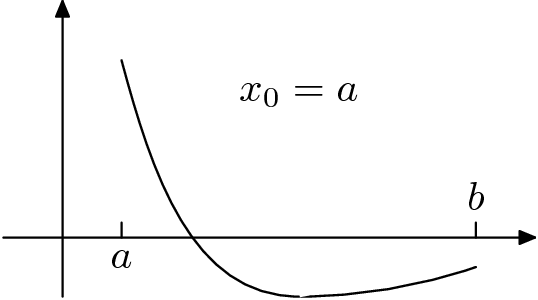
\includegraphics[width=.45\linewidth]{mal-2.png}
	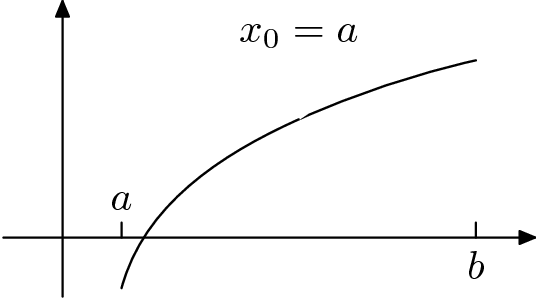
\includegraphics[width=.45\linewidth]{mal-3.png}
\end{figure}

\begin{remark}
	Якщо $\overline{x}$ -- $p$-кратний корінь тобто $f^{(m)} (x) = 0$, $m = \overline{0,p-1}$, $f^{ (p)} (x) \ne 0$, то в методі Ньютона необхідна наступна модифікація \[x_{k+1} = x_k - p\dfrac{f(x_k)}{f'(x_k)} \quad \text{і} \quad q = \dfrac{M_{p+1}\cdot|x_0-\overline{x}|}{m_p \cdot (p+1)}<1.\]
\end{remark}

\begin{remark}
Метод Ньютона можна застосовувати і для обчислення комплексного кореня, тоді ітераційний процес має вигляд \[z_{k+1} = z_k - \dfrac{f(z_k)}{f'(z_k)}, \quad k = 0,1,\ldots.\] В теоремі про збіжність $q = \frac{|z_0-\overline{z}|\cdot M_2}{2m_1}$, де $m_1 = \Min_{z\in U_r} |f'(z)|$, $M_2 = \Max_{z\in U_r} |f''(z)|$. Тут $|z|$ -- модуль комплексного числа $z$.
\end{remark}

Переваги методу Ньютона: 
\begin{enumerate}
\item висока швидкість збіжності;
\item узагальнюється на системи рівнянь; 
\item узагальнюється на комплексні корені.
\end{enumerate}
Недоліки методу Ньютона: 
\begin{enumerate}
	\item на кожній ітерації обчислюється не тільки $f (x_k )$ , а і похідна $f'(x_k)$;
	\item  збіжність залежить від початкового наближення $x_0$, так як від нього залежить умова збіжності $q = \frac{M_2\cdot |x_0-\overline{x}|}{2m_1} < 1$;
	\item потрібно, щоб $f (x)\in C^{(2)}([a,b])$.
\end{enumerate}
% \subsubsection{Характеристики розсіювання значень}
Нехай маємо вибірку об'єму $n$ спостережень $x_1$, $x_2$, $\ldots$, $x_n$ над випадковою величиною $\xi$.
\begin{enumerate}
	\item \textit{Дисперсія} $D\xi = M(\xi - M\xi)^2$. Вибіркове значення \[ S^2(n) = \dfrac{1}{n-1} \sum_{i=1}^n (x_i - \bar{x}(n))^2 = \dfrac{1}{n-1} \left(\sum_{i=1}^n x_i^2 - n\bar{x}^2(n) \right). \]
	\item \textit{Стандартне (середньоквадратичне) відхилення} $\sqrt{D\xi}$. Вибіркове значення $S(n)$.
	\item \textit{Коефіцієнт варіацій} $V_\xi = \frac{\sqrt{D\xi}}{M\xi} 100\%$, $M\xi\ne0$. Вибіркове значення $\widehat{V}_\xi(n)=\frac{S(n)}{\bar x(n)} 100\%$.
	\item \textit{Стохастичне розсіювання} (імовірнісне відхилення) -- це половина інтерквартильної широти: $\frac{U_{0.75} - U_{0.25}}{2}$. Вибіркове значення $\frac{\widehat{U}_{0.75} - \widehat{U}_{0.25}}{2}$.
	\item \textit{Розмах (широта) вибірки}: $x_{\max}-x_{\min}$, де $x_{\max}, x_{\min}$ -- найбільше та найменше значення у вибірці.
	\item \textit{Інтервал концентрації} $(M\xi - 3\sqrt{D\xi}, M\xi + 3 \sqrt{D\xi})$. Вибіркове значення $(\bar x(n) - 3S(n), M\bar x(n) + 3 S(n))$.
\end{enumerate}
\subsubsection{Характеристики скошеності та гостроверхості розподілу}
Нехай є розподіл випадкової величини $\xi$ і отримані спостереження $x_1$, $x_2$, $\ldots$, $x_n$ над нею.
\begin{enumerate}
	\item \textit{Коефіцієнт асиметрії} -- характеристика скошеності розподілу (базується на третьому центральному моменті): \[ \beta_1 = \dfrac{M(\xi - M\xi)^3}{(M(\xi - M\xi)^2)^{3/2}}, \quad D\xi > 0. \] Вибіркове значення \[ \widehat{\beta}_1 = \dfrac{\dfrac{1}{n}\Sum_{i=1}^n(x_k - \bar{x}(n))^3}{S^3(n)}. \] Дисперсія спостережуваної величини $D\xi > 0$. \\ % figure 6

	Якщо розподіл симетричний (наприклад нормальний) то $\beta_1 =0$. Якщо $\beta_1 > 0$, то розподіл скошений вліво, якщо $\beta_1 < 0$, то вправо.
	\item \textit{Коефіцієнт ексцесу} -- характеристика гостроверхості розподілу (базується на четвертому центральному моменті): \[ \beta_2 = \dfrac{M(\xi-M\xi)^4}{(M(\xi-M\xi)^2)^2} - 3, \quad D\xi > 0. \] Вибіркове значення \[ \widehat{\beta}_2 = \dfrac{\dfrac{1}{n}\Sum_{i=1}^n(x_k - \bar{x}(n))^4}{S^4(n)} - 3. \]
	Для нормального розподілу коефіцієнт ексцесу дорівнює нулю. Якщо $\beta_2 > 0$, то розподіл більш гостроверхий ніж нормальний, якщо $\beta_2 < 0$ то відповідно менш гостроверхий.
\end{enumerate}
\subsection{Характеристики векторних величин}
Аналіз $q$-вимірних векторних величин, отримано $n$ спостережень над вектором $\vec\xi: x_1, x_2, \ldots, x_n$, $x_i \in \RR^q$, $i = \overline{1,n}$.
\subsubsection{Характеристики положення центру значень}
\begin{enumerate}
	\item \textit{Математичне сподівання} (теоретичне середнє) $M\xi$. Вибіркове значення \[\bar{x}(n) = \dfrac{1}{n} \Sum_{i=1}^n \vec{x}_i.\]
	\item \textit{Мода} $x_{\text{mod}}$. У неперервному випадку -- це точка максимуму функції щільності $\xi$. Для дискретного випадку -- це значення, яке набуває $\xi$ з найбільшою ймовірністю.
\end{enumerate}
\subsubsection{Характеристики розсіювання значень}
\begin{enumerate} 
	\item \textit{Коваріаційна матриця} $\sum = M(\xi - M\xi)(\xi - M\xi)^T$. Вибіркове значення \[\widehat{\sum}(n) = \dfrac{1}{n-1} \Sum_{k=1}^n (x_k - \bar x(n))(x_k - \bar x(n))^T.\]
	\item \textit{Узагальнена дисперсія} -- визначник коваріаційної матриці: $\det \sum$. Вибіркове значення $\det\left(\widehat{\sum}\right)$.
	\item \textit{Слід коваріаційної матриці} $\trace\sum$. Вибіркове значення $\trace\left(\widehat{\sum}(n)\right)$.
\end{enumerate}
\subsection{Перевірка стохастичності вибірки}
Перевіряємо, чи справді вибірка є випадковою, а не знаходиться під впливом деякого систематичного зміщення. Для цього запропоновано критерії:
\begin{itemize}
	\item Критерій серій на базі медіани
	\item Критерій зростаючих та спадаючих серій
	\item Критерій квадратів послідовних різниць (критерій Аббе)
\end{itemize}
Нехай $x_1$, $x_2$, $\ldots$, $x_n$ -- вибірка спостережень, яка досліджується. \\

Будемо перевіряти гіпотезу $H_0$: ця вибірка є стохастичною з рівнем значимості $\alpha (0 < \alpha < 1$) (рівень значимості -- ймовірність допустити помилку першого роду).
\begin{enumerate}
	\item \textit{Критерій серій на базі медіани}. Альтернативна гіпотеза $H_1$: наявність у вибірці систематичного монотонного зміщення середнього. \\

	Спочатку визначається вибіркове значення медіани $\widehat{x}_{\text{med}}$. Потім під кожним членом вибірки ставимо відповідно \[ \begin{cases} +, & x_i > \widehat{x}_{\text{med}} \\
 \text{нічого}, & x_i = \widehat{x}_{\text{med}} \\
 -, & x_i < \widehat{x}_{\text{med}} \end{cases}. \]
	Отримаємо послідовність символів. \textit{Серія} -- послідовність підряд розташованих однакових символів $+$ чи $-$. \textit{Довжина серії} -- це кількість членів у ній. \\

	Для отриманої послідовності обчислюємо дві статистики: загальну кількість серій в послідовності $v(n)$, довжину найдовшої серії $\tau(n)$. Запишемо область прийняття нашої гіпотези: \[ \left\{ \begin{matrix} v(n) > v_\beta(n) \\
 \tau(n) < \tau_{1-\beta}(n) \end{matrix} \right. \] 
	де $v_\beta(n)$, $\tau_\beta(n)$ -- квантилі рівня $\beta$ статистик $v(n)$, $\tau(n)$ відповідно. При фіксованому значенні $\beta$ рівень значимості $\alpha$ лежить у межах $\beta < \alpha < 2\beta - \beta^2$. Якщо порушується хоч одна з нерівностей, то гіпотеза відхиляється.
	\item \textit{Критерій зростаючих та спадаючих серій}. Альтернативна гіпотеза $H_1$: наявність у вибірці систематичного періодичного зміщення середнього. Спочатку у вибірці замінюємо підряд розташовані однакові виміри одним їх представником. В результаті отримаємо послідовність $x_1'$, $x_2'$, $\ldots$, $x_k'$. Під кожним членом послідовності ставимо відповідно \[ \begin{cases} +, & x_i' < x_{i+1}' \\
 -, & x_i' > x_{i+1}' \end{cases}. \]
	Далі для таким чином отриманої послідовності $+$ та $-$, як і в попередньому випадку, обчислюємо дві статистики: загальну кількість серій в послідовності $v(n)$, довжину найдовшої серії $\tau(n)$. Запишемо область прийняття нашої гіпотези: \[ \left\{ \begin{matrix} v(n) > v_\beta(n) \\
 \tau(n) < \tau_{1-\beta}(n) \end{matrix} \right. \] де $v_\beta(n)$, $\tau_\beta(n)$ -- квантилі рівня $\beta$ статистик $v(n)$, $\tau(n)$ відповідно. При фіксованому значенні $\beta$ рівень значимості $\alpha$ лежить у межах $\beta < \alpha < 2\beta - \beta^2$. Якщо порушується хоч одна з нерівностей, то гіпотеза відхиляється.
	\item \textit{Критерій квадратів послідовних різниць (критерій Аббе)}. Він є найбільш потужним на класі усіх нормальних вибірок. Альтернативна гіпотеза $H_1$: наявність у вибірці систематичного зміщення середнього. \\

	На основі вибірки підраховуємо наступну статистику: \[ \gamma(n) = \dfrac{\dfrac{1}{2(n-1)} \Sum_{i=1}^{n-1} (x_{i+1}-x_i)^2}{\dfrac{1}{n-1}\left(\Sum_{i=1}^n x_i^2 - n \bar{x}^2(n)\right)}. \]
	Область прийняття гіпотези для цього критерію має вигляд $\gamma(n) > \gamma_\alpha(n)$, де $\gamma_\alpha(n)$ -- квантиль рівня $\alpha$ статистики $\gamma(n)$, що при $n \le 60 $визначається з таблиць, а протилежному випадку потрібно скористатися формулою \[\gamma_\alpha(n) = 1 + \dfrac{u_\alpha}{\sqrt{n + 0.5(1 + u_\alpha^2)}}, \] де $u_\alpha$ -- квантиль рівня $\alpha$ нормального розподілу з параметрами 0 та 1.
\end{enumerate}
% \section{Ітераційні методи для систем}

\subsection{Ітераційні методи розв'язання СЛАР}

Систему
\begin{equation}
	\label{eq:4.1}
	A \vec x = \vec b
\end{equation}
зводимо до вигляду
\begin{equation}
	\label{eq:4.2}
	\vec x = B \vec x + \vec f.
\end{equation}
Будь яка система
\begin{equation}
	\label{eq:4.3}
	\vec x = \vec x - C \cdot (A \vec x - \vec b)
\end{equation}
має вигляд (\ref{eq:4.2}) і при $\det C \ne 0$ еквівалентна системі (\ref{eq:4.1}). Наприклад, для $C = \tau \cdot E$:
\begin{equation}
	\label{eq:4.4}
	\vec x = \vec x - \tau \cdot (A \vec x - \vec b).
\end{equation}


\subsubsection{Метод простої ітерації}

Цей метод застосовується до рівняння (\ref{eq:4.2})
\begin{equation}
	\label{eq:4.5}
	\vec x^{(k+1)} = B \vec x^{(k)} + \vec f,
\end{equation}
де $\vec x^{(0)}$ -- початкове наближення, задано.\\

Ітераційний процес збігається, тобто $\left\| \vec x^{(k)} - \vec x\right\| \xrightarrow[k\to\infty]{} 0$, якщо
\begin{equation}
	\label{eq:4.6}
	\|B\| \le q < 1
\end{equation}
При цьому має місце оцінка
\begin{equation}
	\label{eq:4.7}
	\left\|\vec x^{(n)} - \vec x\right\| \le \dfrac{q^n}{1-q}\cdot\left\|\vec x^{(1)} - \vec x^{(0)}\right\|.
\end{equation}

\subsubsection{Метод Якобі}

Припустимо $\forall i$: $a_{i,i} \ne 0$. Зведемо систему (\ref{eq:4.1}) до вигляду
\[ x_i = -\Sum_{j=1}^{i-1} \dfrac{a_{i,j}}{a_{i,i}} \cdot x_j - \Sum_{j=i+1}^n \dfrac{a_{i,j}}{a_{i,i}} \cdot x_j + \dfrac{b_i}{a_{i,i}}, \quad i=\overline{1,n}. \]

Ітераційний процес запишемо у вигляді
\begin{equation}
	\label{eq:4.8}
	x_i^{(k+1)} = -\Sum_{j=1}^{i-1} \dfrac{a_{i,j}}{a_{i,i}} \cdot x_j^{(k)} - \Sum_{j=i+1}^n \dfrac{a_{i,j}}{a_{i,i}} \cdot x_j^{(k)} + \dfrac{b_i}{a_{i,i}}, \quad k = 0,1,\ldots, \quad i=\overline{1,n}.
\end{equation}

Ітераційний процес збігається до розв’язку, якщо виконується умова
\[ \forall i: \Sum_{\substack{j = 1 \\ i \ne j}}^n |a_{i,j}| \le |a_{i,i}|. \]

Це умова діагональної переваги матриці $A$. Якщо ж
\begin{equation}
	\label{eq:4.9}
	\forall i: \Sum_{\substack{j = 1 \\ i \ne j}}^n |a_{i,j}| \le q\cdot|a_{i,i}|, \quad 0 \le q < 1.
\end{equation}
то має місце оцінка точності:
\[ \|\vec x^{(n)} - \vec x\| \le \dfrac{q^n}{1-q}\cdot\|\vec x^{(0)}-\vec x\|. \]

\subsubsection{Метод Зейделя}
В компонентному вигляді ітераційний метод Зейделя записується так:
\begin{equation}
	\label{eq:4.10}
	x_i^{(k+1)} = -\Sum_{j=1}^{i-1} \dfrac{a_{i,j}}{a_{i,i}} \cdot x_j^{(k+1)} - \Sum_{j=i+1}^n \dfrac{a_{i,j}}{a_{i,i}} \cdot x_j^{(k)} + \dfrac{b_i}{a_{i,i}}, \quad k = 0,1,\ldots, \quad i=\overline{1,n}.
\end{equation}

На відміну від методу Якобі на $k$-му-кроці попередні компоненти розв'язку беруться з $k+1$-ої ітерації. \\

Достатня умова збіжності методу Зейделя -- $A^T = A > 0$.

\subsubsection{Матрична інтерпретація методів Якобі і Зейделя}

Подамо матрицю $A$ у вигляді \[ A = A_1 + D + A_2, \]
де $A_1$ -- нижній трикутник матриці $A$, $A_2$ -- верхній трикутник матриці $A$, $D$ -- її
діагональ. Тоді систему (\ref{eq:4.1}) запишемо у вигляді \[ D \vec x = A_1 \vec x + A_2 \vec x + \vec b,\]
або
\[ \vec x = D^{-1} A_1 \vec x + D^{-1} A_2 \vec x + D^{-1} \vec b,\]
 
Матричний запис методу Якобі:
\[ \vec x^{(k+1)} = D^{-1} A_1 \vec x^{(k)} + D^{-1} A_2 \vec x^{(k)} + D^{-1} \vec b,\]
методу Зейделя:
\[ \vec x^{(k+1)} = D^{-1} A_1 \vec x^{(k+1)} + D^{-1} A_2 \vec x^{(k)} + D^{-1} \vec b,\]

Необхідна і достатня умова збіжності методу Якобі: всі корені рівняння \[\det(D + \lambda(A_1 + A_2 )) = 0\] по модулю більше 1. \\

Необхідна і достатня умова збіжності методу Зейделя: всі корені рівняння \[\det(A_1 + D + \lambda A_2) = 0\] по модулю більше 1.

\subsubsection{Однокрокові (двошарові) ітераційні методи}

Канонічною формою однокрокового ітераційного методу розв'язку СЛАР є його запис у вигляді
\begin{equation}
	\label{eq:4.11}
	B_k \dfrac{\vec x^{(k+1)} - \vec x^{(k)}}{\tau_{k+1}} + A \vec x^{(k)} = \vec b,
\end{equation}

Тут $\{B_k\}$ -- послідовність матриць (пере-обумовлюючі матриці), що задають ітераційний метод на кожному кроці; $\{\tau_{k+1}\}$ -- ітераційні параметри. \\

Якщо $B_k = E$, то ітераційний процес називається \textit{явним}
\[ \vec x^{(k+1)} = \vec x^{(k)} - \tau_{k+1} \left(A \vec x^{(k)} + \vec b\right). \]
Якщо $B_k \ne E$, то ітераційний процес називається \textit{неявним}
\[ B_k \vec x^{(k+1)} = F^k. \]

У цьому випадку на кожній ітерації необхідно розв'язувати СЛАР. \\

Якщо $\tau_{k+1} \equiv \tau$, $B_k \equiv B$, то ітераційний процес називається \textit{стаціонарним}; інакше -- \textit{нестаціонарним}. \\

Методам, що розглянуті вище відповідають:
\begin{itemize}
	\item методу простої ітерації: $B_k = E$, $\tau_{k+1} = \tau$;
	\item методу Якобі: $B_k = D$, $\tau_{k+1} = 1$.;
	\item методу Зейделя: $B_k = D + A_1$, $\tau_{k+1} = 1$.
\end{itemize}

\subsubsection{Збіжності стаціонарних ітераційних процесів у випадку симетричних матриць}

Розглянемо випадок симетричних матриць $A^T=A$ і стаціонарний ітераційний процес $B_k \equiv E$, $\tau_{k+1} \equiv \tau$. \\

Нехай для $A$ справедливі нерівності
\begin{equation}
	\label{eq:4.12}
	\gamma_1 E \le A \le \gamma_2 E, \quad \gamma_1, \gamma_2 > 0.
\end{equation}

Тоді при виборі $\tau = \tau_0 = \frac{2}{\gamma_1 + \gamma_2}$ ітераційний процес збігається. Найбільш точним значенням $\gamma_1$, $\gamma_2$ при яких виконуються обмеження (\ref{eq:4.12}) є $\gamma_1 = \min \lambda_i(A)$, $\gamma_2 = \max \lambda_i(A)$. Тоді 
\[q = q_0 = \dfrac{\gamma_2 - \gamma_1}{\gamma_2 + \gamma_1} = \dfrac{1-\xi}{1+\xi}, \quad \xi = \dfrac{\gamma_1}{\gamma_2}.\]
(Зауважимо, що аналогічно обчислюється $q$ і для методу релаксації розв'язання нелінійних рівнянь, де $\gamma_1 = m = \min |f'(x)|$, $\gamma_2 = M_1 = \max|f'(x)|$) і справедлива оцінка\[ \|\vec x^{(n)} - \vec x\| \le \dfrac{q^n}{1-q} \cdot \|\vec x^{(0)} - \vec x\|. \]

Явний метод з багатьма параметрами $\{\tau_k\}$:
\[ B \equiv E, \quad \{\tau_k\}: \Min_\tau q(\tau), \quad n=n(\epsilon)\to\min,\]
які обчислюються за допомогою нулів багаточлена Чебишова, називаються ітераційним методом з чебишевським набором параметрів.

\subsubsection{Метод верхньої релаксації}

Узагальненням методу Зейделя є метод верхньої релаксації: \[ (D + \omega A_1) \cdot\dfrac{\vec x^{(k+1)} + \vec x^{(k)}}{\omega} + A \vec x^{(k)} = \vec b,\]
де $D$ -- діагональна матриця з елементами $a_{i,i}$ по діагоналі. $\omega > 0$ -- заданий числовий параметр. \\

Тепер $B = D + \omega A_1$, $\tau = \omega$. Якщо $A^T = A > 0$, то метод верхньої релаксації збігається при умові $0 < \omega < 2$. Параметр підбирається експериментально з умови мінімальної кількості ітерацій. 

\subsubsection{Методи варіаційного типу}

До цих методів відносяться: метод мінімальних нев’язок, метод мінімальних поправок, метод найшвидшого спуску, метод спряжених градієнтів. Вони дозволяють обчислювати наближення без використання апріорної інформації про $\gamma_1$, $\gamma_2$ в (\ref{eq:4.12}). \\

Нехай $B = E$. Для методу мінімальних нев’язок параметри $\tau_{k+1}$ обчислюються з умови 
\[ \left\|\vec r^{(k+1)}\right\|^2 = \left\|\vec r^{(k)}\right\|^2 - 2\tau_{k+1}\cdot\left(\vec r^{(k)}, A\vec r^{(k)}\right) + \tau_{k+1}^2 \cdot\left\|A\vec r^{(k)}\right|^2 \to \min. \]

Тому \[ \tau_{k+1} = \dfrac{\left(A\vec r^{(k)}, \vec r^{(k)}\right) }{\left\|\vec r^{(k)}\right\|^2},\] 
де $\vec r^{(k)} = A \vec x^{(k)} - \vec b$ -- нев'язка. \\

Умова для завершення ітераційного процесу: \[ \left\|\vec r^{(n)}\right\| < \epsilon.\]

Швидкість збіжності цього методу співпадає із швидкістю методу простої ітерації з одним оптимальним параметром $\tau_0 = \frac{2}{\gamma_1+\gamma_2}$. \\

Аналогічно будуються методи з $B \ne E$. Матриця $B$ називається переобумовлювачем і дозволяє підвищити швидкість збіжності ітераційного процесу. Його вибирають з умов 
\begin{enumerate}
	\item легко розв’язувати СЛАР $B \vec x^{(k)} = F_k$ (діагональний, трикутній, добуток трикутніх та інше); 
	\item зменшення числа обумовленості матриці $B^{-1}A$ у порівнянні з $A$.
\end{enumerate}

\subsection{Методи розв’язання нелінійних систем}

Розглянемо систему рівнянь
\[ \left\{ \begin{aligned} & f_1(x_1, \ldots, x_n) = 0, \\ & \ldots \\ & f_n(x_1,\ldots,x_n) = 0. \end{aligned} \right. \]

Перепишемо її у векторному вигляді: 
\begin{equation}
	\label{eq:4.13}
	\vec f(\vec x) = 0.
\end{equation}

\subsubsection{Метод простої ітерації}

В цьому методі рівняння (\ref{eq:4.13}) зводиться до еквівалентного вигляду
\begin{equation}
	\label{eq:4.14}
	\vec x = \vec \Phi(\vec x).
\end{equation}

Ітераційний процес представимо у вигляді:
\begin{equation}
	\label{eq:4.15}
	\vec x^{(k+1)} = \vec \Phi\left(\vec x^{(k)}\right).
\end{equation}
початкове наближення $\vec x^{(0)}$ -- задано. \\

Нехай оператор $\vec \Phi$ визначений на множині $H$. За теоремою про стискуючі відображення ітераційний процес (\ref{eq:4.15}) сходиться, якщо виконується умова
\begin{equation}
	\label{eq:4.16}
	\left\| \vec \Phi(\vec x) - \vec \Phi(\vec y) \right\| \le q \cdot \|\vec x - \vec y\|, \quad 0 < q < 1, 
\end{equation}
або
\begin{equation}
	\label{eq:4.17}
	\left\| \vec \Phi'(\vec x)\right\| \le q < 1, 
\end{equation}
де $\vec x\in U_r$, $\vec \Phi'(\vec x) = \left(\frac{\partial \phi_i}{\partial x_j}\right)_{i,j=1}^n$. Для похибки справедлива оцінка
\[ \left\| \vec x^{(m)} - \vec x\right\| \le \dfrac{q^n}{1 - q} \cdot\left\|\vec x^{(0)} - \vec x\right\|.\]

Частинним випадком методу простої ітерації є метод релаксації для рівняння (\ref{eq:4.13}):
\[ \vec x^{(k+1)} = \vec x^{(k)} - \tau \cdot \vec F\left(\vec x^{(k)}\right), \]
де $\tau < \frac{2}{\left\|\vec F'(\vec x)\right\|}$.

\subsubsection{Метод Ньютона}

Розглянемо рівняння
\[ \vec F(\vec x) = 0. \]

Представимо його у вигляді
\begin{equation}
	\label{eq:4.18}
	\vec F\left(\vec x^{(k)}\right) + \vec F'\left(\vec \xi^{(k)}\right)\cdot\left(\vec x - \vec x^{(k)}\right) = 0,
\end{equation}
де $\vec \xi^{(k)} = \vec x^{(k)} + \theta_k \cdot \left(\vec x^{(k)} - \vec x\right)$, $0 < \theta_k < 1$. Тут  $\vec F'(\vec x) = \left(\frac{\partial f_i}{\partial x_j}\right)_{i,j=1}^n$ -- матриця Якобі для $\vec F(\vec x)$. Можемо наближено вважати $\vec \xi^{(k)} \approx \vec x^{(k)}$. Тоді з (\ref{eq:4.18}) матимемо
\begin{equation}
	\label{eq:4.19}
	\vec F\left(\vec x^{(k)}\right) + \vec F'\left(\vec x^{(k)}\right) \cdot\left(\vec x^{(k+1)} - \vec x^{(k)}\right) = 0.
\end{equation}
Ітераційний процес представимо у вигляді:
\begin{equation}
	\label{eq:4.20}
	\vec x^{(k+1)} = \vec x^{(k)} - \vec F'\left(\vec x^{(k)}\right)^{-1} \cdot \vec F\left(\vec x^{(k)}\right). 
\end{equation}

Для реалізації методу Ньютона потрібно, щоб існувала обернена матриця \[\vec F'\left(\vec x^{(k)}\right)^{-1}. \]

Можна не шукати обернену матрицю, а розв’язувати на кожній ітерації СЛАР
\begin{equation}
	\label{eq:4.21}
	\left\{
		\begin{aligned}
			& A_k \vec z^{(k)} = \vec F\left(\vec x^{(k)}\right), \\
			& \vec x^{(k + 1)} = \vec x^{(k)} - \vec z^{(k)},
		\end{aligned}
		\quad k=0,1,2,\ldots
	\right.
\end{equation}
де $\vec x^{(0)}$ -- задано, а матриця $A_k = \vec F'\left(\vec x^{(k)}\right)$. \\

Метод має квадратичну збіжність, якщо добре вибрано початкове наближення. Складність методу (при умові використання методу Гаусса розв'язання СЛАР (\ref{eq:4.21}) на кожній ітерації $Q_n = \frac23 n^3+O(n^2)$, де $n$ -- розмірність системи (\ref{eq:4.13}).

\subsubsection{Модифікований метод Ньютона}

Ітераційний процес має вигляд :
\[ \vec x^{(k+1)} = \vec x^{(k)} - \vec F'\left(\vec x^{(0)}\right)^{-1} \cdot\vec F\left(\vec x^{(k)}\right). \]

Тепер обернена матриця обчислюється тільки на нульовій ітерації. На інших -- обчислення нового наближення зводиться до множення матриці $A_0 = \vec F'\left(\vec x^{(0)}\right)^{-1}$ на вектор $\vec F\left(\vec x^{(k)}\right)$ та додавання до $\vec x^{(k)}$. \\

Запишемо метод у вигляді системи лінійних рівнянь (аналог (\ref{eq:4.21}))
\begin{equation}
	\label{eq:4.22}
	\left\{
		\begin{aligned}
			& A_0 \vec z^{(k)} = \vec F\left(\vec x^{(k)}\right), \\
			& \vec x^{(k + 1)} = \vec x^{(k)} - \vec z^{(k)},
		\end{aligned}
		\quad k=0,1,2,\ldots
	\right.
\end{equation}
Оскільки матиця $A_0$ розкладається на трикутні (або обертається) один раз, то складність цього методу на одній ітерації (окрім нульової) $Q_n = O(n^2)$. Але цей метод має лінійну швидкість збіжності. \\

Можливе циклічне застосування модифікованого методу Ньютона, тобто коли обернену матрицю похідних шукаємо та обертаємо через певне число кроків ітераційного процесу. \\

\begin{problem}
	Побудувати аналог методу січних для систем нелінійних рівнянь.
\end{problem}

 \setcounter{section}{2}
 \setcounter{subsection}{4}
 \setcounter{subsubsection}{4}
 \setcounter{theorem}{15}
 \setcounter{equation}{41}

\subsubsection{Додатньо визначені ядра}

\begin{definition}[додатно-визначеного ядра]
    Неперервне ядро $K(x, y)$ називається \it{додатно-визначеним}, якщо $\forall f \in L_2(G)$: $(\bf{K}f, f) \ge 0$,прричому $(\bf{K}f, f) = 0 \iff \|f\|_{L_2(G)} = 0$.
\end{definition}

\begin{remark}
    Довільне додатньо визначене ядро є ермітовим (його білінійна форма $(\bf{K}f, f)$ приймає дійсні значення).
\end{remark}

\begin{lemma}
    Для того, щоб неперервне ядро було додатньо визначеним необхідно і достатньо, щоб його характеристичні числа були додатні.
\end{lemma}

\begin{proof}
    Необхідність: для власних функцій $(\bf{K} \phi_k, \phi_k) = 1 / \lambda_k > 0$. \medskip

    Достатність: Розглянемо $\bf{K} f$ як джерелувато-зображувану функцію, згідно до теореми Гілберта-Шмідта
    \begin{equation}
        \bf{K} f = \sum_{k = 1}^\infty \frac{(f, \phi_k)}{\lambda_k} \phi_k,
    \end{equation}
    тоді 
    \begin{equation}
        (\bf{K}f, f) = \Sum_{k = 1}^\infty \dfrac{(f, \phi_k)}{\lambda_k} (\phi_k, f) = \Sum_{k = 1}^\infty \dfrac{|(f, \phi_k)|^2}{\lambda_k} > 0,
    \end{equation}
    отже квадратична форма додатньо визначена. \medskip

    Таким чином додатність характеристичних чисел є критерієм додатної визначеності ядра.
\end{proof}

\begin{lemma}
    Довільне додатньо визначене неперервне ядро має характеристичні числа і для них має місце варіаційний принцип:
    \begin{equation}
        \dfrac{1}{\lambda_k} = \Sup_{\substack{f \in L_2(G) \\ (f, \phi_i) = 0, i = \overline{1, k - 1}}} \dfrac{(\bf{K}f, f)_{L_2(G)}}{\|f\|_{L_2(G)}^2}, \quad k = 1, 2, \ldots,
    \end{equation}
    де $\lambda_1 \le \lambda_2 \le \lambda_3 \le \ldots$, а $\phi_1, \phi_2, \phi_3, \ldots$ --- ортонормована система власних функцій.
\end{lemma}

\begin{proof}
    З теореми Гілберта Шмідта можна оцінити 
    \begin{equation}
        \dfrac{(\bf{K}f, f)_{L_2(G)}}{\|f\|_{L_2(G)}^2} = \Sum_{i=k}^\infty \dfrac{|(f, \phi_i)|^2}{\lambda_i\|f\|^2} \le \dfrac{1}{\lambda_k} \Sum_{i=k}^\infty \dfrac{|(f, \phi_i)|^2}{\|f\|^2} \le \dfrac{1}{\lambda_k}.
    \end{equation}
    (перша нерівність виконується оскільки $\lambda_k$ --- найменше характеристичне число в сумі, а друга випливає з нерівності Бесселя). \medskip

    З іншого боку при $f = \phi_k$ маємо
    \begin{equation}
        \frac{(\bf{K}\phi_k, \phi_k)}{\|\phi_k\|^2} = \frac{1}{\lambda_k},
    \end{equation}
    тобто існує функція на якій досягається верхня межа цієї нерівності.
\end{proof}

\begin{theorem}[Мерсера, про регулярну збіжність білінійного ряду для ермітових ядер зі скінченою кількістю від'ємних характеристичних чисел] 
    Якщо ермітове неперервне ядро $K(x, y)$ має лише скінчену кількість від'ємних характеристичних чисел, то його білінійний ряд 
    \begin{equation}
        K(x,y)=\Sum_{i=1}^\infty\dfrac{\phi_i(x)\overline\phi_i(y)}{\lambda_i}
    \end{equation}
    збігається в $\overline G\times\overline G$ абсолютно і рівномірно.
\end{theorem}

\begin{proof}
    Покажемо, що якщо ядро $K(x,y)$ --- додатньо визначене, то $\forall x\in\overline G$: $K(x,x)\ge0$. Оскільки $K(x,y)$ --- ермітове, то $K(x,x)=\overline {K(x,x)}$ і є дійсною функцією. Якщо існує хоча б одна точка $x_0\in\overline G$ така, що $K(x_0,x_0)<0$, то виходячи з неперервності знайдеться і деякій окіл цієї точки $U(x_0,x_0)\subset\overline G\times\overline G$ такий, що $\forall(x,y)\in U(x_0,x_0)$: $\text{Re} K(x,y)<0$. Оберемо невід'ємну неперервну функцію $\phi(x)$ яка відміна від нуля лише в $U(x_0,x_0)$ і отримаємо
    \begin{equation}
        \begin{aligned}
            (\bf{K}\phi,\phi)&=\Int_{U(x_0,x_0)}K(x,y)\phi(x)\phi(y)\diff x\diff y=\\
            &=\Int_{U(x_0,x_0)}\text{Re}K(x,y)\phi(x)\phi(y)\diff x\diff y\le0.
        \end{aligned}
    \end{equation}

    Остання нерівність вступає в протиріччя з припущенням додотньої визначеності ядра, тобто теорему достатньо довести для додатньо визначених ядер. \medskip

    Розглянемо ядро
    \begin{equation}
        K^p(x,y)=K(x,y)-\sum_{i=1}^p\frac{\overline\phi_i(y)\phi_i(x)}{\lambda_i},
    \end{equation}
    де $p$ --- номер останнього від'ємного характеристичного числа, так що усі $\lambda_i$, $i=p+1,p+2,\ldots$ є додатніми. Таким чином ядро $K^p(x,y)$ є неперервним та додатньо визначеним. А це означає, що $\forall x\in\overline G:K^p(x,x)\ge0$. Таким чином маємо нерівність:
    \begin{equation}
        \Sum_{i=1}^N\dfrac{|\phi_i(x)|^2}{\lambda_i}\le K(x,x)\le M,\quad x\in\overline G, N=p+1,p+2,\ldots,
    \end{equation}
    тобто ряд
    \begin{equation}
        \sum_{k=1}^\infty\frac{|\phi_k(x)|^2}{\lambda_k}
    \end{equation}
    рівномірно збіжний. \medskip

    Розглянемо білінійний ряд 
    \begin{equation}
        \sum_{i=1}^\infty\frac{\phi_i(x)\overline\phi_i(y)}{\lambda_i}
    \end{equation}
    і доведемо його абсолютну і рівномірну збіжність за критерієм Коші. Використовуючи нерівність Коші-Буняківського маємо:
    \begin{equation}
        \Sum_{k=p}^{p+q}\dfrac{|\phi_k(x)\overline\phi_k(y)|}{\lambda_k}\le\left(\Sum_{k=p}^{p+q}\dfrac{|\phi_k(x)|^2}{\lambda_k}\cdot\Sum_{k=p}^{p+q}\dfrac{|\phi_k(y)|^2}{\lambda_k}\right)^{1/2}
    \end{equation}

    Але оскільки
    \begin{equation}
        \sum_{k=1}^\infty\frac{|\phi_k(x)|^2}{\lambda_k}
    \end{equation}
    рівномірно збіжний, то білінійний ряд
    \begin{equation}
        K(x,y)=\Sum_{i=1}^\infty\dfrac{\phi_i(x)\overline\phi_i(y)}{\lambda_i}
    \end{equation}
    збігається абсолютно і рівномірно (регулярно) в $\overline G\times\overline G$.
\end{proof}

\begin{remark}
    Теорема Гільберта-Шмідта і її наслідки, встановлені для ермітового неперервного ядра, залишаються вірними і для ермітового слабо полярного ядра.
\end{remark}

\begin{remark}
    Теорема Гільберта-Шмідта і формула Шмідта у випадку полярного ядра залишаються вірними, але з заміною рівномірної збіжності на середньоквадратичну.
\end{remark}

\subsection{Задача Штурма-Ліувілля. Теорема Стеклова}

Постановка задачі Штурма-Ліувілля: нехай $\bf{L}$ --- диференціальний оператор другого порядку: задано рівняння
\begin{equation}
    \label{eq:2.5.1}
    \bf{L}u=(-p(x)u')'+q(x)u=\lambda u,\quad0<x<l,
\end{equation}
з крайовими умовами
\begin{align}
    \label{eq:2.5.2}
    l_1(u)|_{x=0}&=h_1u(0)-h_2u'(0)=0,\\
    \label{eq:2.5.3}
    l_2(u)|_{x=l}&=H_1u(l)+H_2u'(l)=0,
\end{align}
де функція $p\in C^{(1)}([0,l])$, $p>0$, функція $q\in C([0,l])$, $q\ge0$, виконуються наступні умови на сталі: $h_1, h_2, H_1, H_2 \ge 0$, $h_1+h_2>0$, $H_1+H_2>0$,
а також
\begin{equation}
    \label{eq:2.5.4}
    M_L=\{u:u\in C^{(2)}(0,l)\cap C^{(1)}([0,l]), u''\in L_2(0,l), l_1u(0)=l_2u(l)=0\}
\end{equation}
-- область визначення оператора $\bf{L}$.

\begin{definition}[власних чисел і функцій задачі Штурма-Ліувілля]
    Знайти розв'язки задачі Штурма-Ліувіля означає знайти всі ті значення параметра $\lambda$, при яких крайова задача \eqref{eq:2.5.1}--\eqref{eq:2.5.4} має нетривіальний розв'язок. Ці значення називаються \it{власними значеннями} задачі Штурма-Ліувіля, а самі розв'язки --- \it{власними функціями}.
\end{definition}

\subsubsection{Функція Гріна оператора $\bf{L}$}

Будемо припускати, що $\lambda = 0$ не є власним числом оператора $\bf{L}$ задачі Штурма-Ліувіля. \medskip

Розглянемо крайову задачу:
\begin{system}
    & (-p(x)u')'+q(x)u=f(x),\quad0<x<l \\
    & l_1(u)|_{x=0}=l_2(u)|_{x=l}=0
\end{system}

Припустимо що $f \in C(0,l)\cap L_2(0,l)$. \medskip

З припущення, що $\lambda = 0$ не є власним числом випливає, що задача має єдиний розв'язок. \medskip

Розглянемо функції $v_i(x)$, $i=1,2$ --- ненульові дійсні розв'язки однорідних задач Коші:
\begin{system}
    & (-p(x)v_i'(x))'+q(x)v_i'(x)=0,\quad i=1,2 \\
    & l_1v_1|_{x=0}=l_2v_2|_{x=l}=0
\end{system}

З загальної теорії задач Коші випливає, що розв'язки цих задач Коші існують, тому $v_i(x)$ --- двічі неперервно диференційовані функції.

\begin{proposition}
    $v_1(x)$, $v_2(x)$ --- лінійно незалежні.
\end{proposition}

\begin{proof}
    Припустимо що це не так і $v_1(x) = cv_2(x)$, тобто $v_1(x)$ задовольняє одночасно граничним умовам на лівому і правому краях. Тоді $v_1(x)$ --- власна функція оператора $\bf{L}$, і відповідає власному числу $\lambda = 0$ що суперечить припущенню.
\end{proof}

В цьому випадку визначник Вронського
\begin{equation}
    w(x) = \begin{vmatrix} v_1 & v_2 \\ v_1' & v_2' \end{vmatrix} \ne 0
\end{equation}

Будемо шукати розв'язок задачі методом варіації довільної сталої у вигляді:
\begin{equation}
    u(x) = c_1(x) v_1(x) + c_2(x) v_2(x).
\end{equation}

Підставимо в рівняння:
\begin{equation}
    (-p(c_1'v_1+c_2'v_2+c_1v_1'+c_2v_2')'+q(c_1v_1+c_2v_2)=f.
\end{equation}

Накладемо першу умову на коефіцієнти: $c_1'v_1+c_2'v_2=0$, маємо: 
\begin{equation}
    -p'(c_1v_1'+c_2v_2')-p(c_1'v_1'+c_2'v_2'+c_1v_1''+c_2v_2'')+q(c_1v_1+c_2v_2)=f,
\end{equation}
або
\begin{equation}
    c_1Lv_1 + c_2Lv_2 - p(c_1'v_1'+c_2'v_2')=f,
\end{equation}
оскільки $c_1\bf{L}v_1=0$, $c_2\bf{L}v_2=0$, то
\begin{equation}
    -p(c_1'v_1'+c_2'v_2')=f,
\end{equation}
отже
\begin{equation}
    c_1'v_1'+c_2'v_2'=-\frac{f}{p}.
\end{equation}

Таким чином $c_1'$ та $c_2'$ повинні задовольняти системі лінійних диференціальних рівнянь:
\begin{system}
    c_1'v_1 + c_2'v_2 &= 0, \\
    c_1'v_1' + c_2'v_2' &= - \dfrac{f}{p},
\end{system}
визначник системи
\begin{equation}
    w(x) = \begin{vmatrix} v_1 & v_2 \\ v_1' & v_2' \end{vmatrix} \ne 0.
\end{equation}

\begin{remark}
    Має місце рівність Ліувілля:
    \begin{equation}
        w(x)\cdot p(x)=w(0)\cdot p(0)=\text{const}.
    \end{equation}
\end{remark}

Розв'язавши систему рівнянь, отримаємо:
\begin{system}
    c_1'(x) &= \dfrac{1}{w(x)} \begin{vmatrix} 0 & v_2 \\ - \dfrac{f}{p} & v_2' \end{vmatrix} = \dfrac{v_2(x)f(x)}{p(0)w(0)}, \\
    c_2'(x) &= \dfrac{1}{w(x)} \begin{vmatrix} v_1 & 0 \\ v_1' & - \dfrac{f}{p} \end{vmatrix} = -\dfrac{v_1(x)f(x)}{p(0)w(0)}, 
\end{system}

Знайдемо додаткові умови для диференціальних рівнянь вище: 
\begin{multline} 
l_1u|_{x=0} = h_1(c_1(0)v_1(0) + c_2(0)v_2(0)) - \\
- h_2(c_1'(0)v_1(0) + c_2'(0)v_2(0) + c_1(0)v_1'(0) + c_2(0)v_2'(0)) = 0,
\end{multline}
а враховуючи, що $c_1'(0)v_1(0)+c_2'(0)v_2(0) = 0$ маємо
\begin{equation}
    c_1(0) (h_1v_1(0) - h_2v_1'(0)) + c_2(0)v_2'(0) = 0.
\end{equation}

Оскільки перший доданок дорівнює нулю, то остання рівність виконується коли $c_2(0) = 0$, аналогічно отримаємо, що $c_1(l) = 0$. \medskip

Проінтегруємо систему дифурів що розглядається, отримаємо
\begin{equation}
    c_1(x)=-\Int_x^l\dfrac{f(\xi)v_2(\xi)}{p(0)w(0)}\diff\xi, \quad c_2(x)=-\Int_0^x\dfrac{v_1(\xi)f(\xi)}{p(0)w(0)}\diff\xi
\end{equation}

Тоді розв'язок крайової задачі буде мати вигляд:
\begin{equation}
    u(x)=-\Int_0^x\dfrac{v_1(\xi)v_2(x)f(\xi)}{p(0)w(0)}\diff\xi-\Int_x^l\dfrac{f(\xi)v_1(x)v_2(\xi)}{p(0)w(0)}\diff\xi
\end{equation}

\begin{definition}[функції Гріна]
    \it{Функція Гріна} визначається наступним чином:
    \begin{equation}
        G(x, \xi) = - \dfrac{1}{p(0)w(0)} \begin{cases}
            v_1(\xi) v_2(x), & 0 \le \xi \le x \le l, \\
            v_1(x) v_2(\xi), & 0 \le x \le \xi \le l.
        \end{cases}
    \end{equation}
\end{definition}

Отже розв'язок крайової задачі можна записати у вигляді
\begin{equation}
    u(x) = \Int_0^l G(x, \xi) f(\xi) \diff \xi
\end{equation}

$G(x, \xi)$ називається функцією Гріна оператора Штурма-Ліувіля. Попередні міркування доводять наступну лемму.
\begin{lemma}
    \label{lemma:2.5.5}
    Якщо $\lambda = 0$ не є власним числом задачі Штурма-Ліувіля, то роз\-в'яз\-ок крайової задачі існує та єдиний і представляється за формулою
    \begin{equation}
        u(x) = \Int_0^l G(x, \xi) f(\xi) \diff \xi
    \end{equation}
    через функцію Гріна.
\end{lemma}

\newpage

\subsubsection{Властивості функції Гріна}
\begin{properties}[функції Гріна]
    Можна показати, що:
    \begin{enumerate}
        \item \begin{itemize}
                \item $G(x, \xi) \in C([0, l] \times [0, l])$;
                \item $G(x, \xi) \in C^{(2)}(0 < x < \xi < l)$;
                \item $G(x, \xi) \in C^{(2)} (0 < \xi < x < l)$.
            \end{itemize}
        \item Симетричність: $G(x, \xi) = G(\xi, x)$, $x, \xi \in [0, l] \times [0, l]$.
        \item На діагоналі $x = \xi$ має місце розрив першої похідної:
            \begin{equation}
                \frac{\partial G(\xi + 0, \xi)}{\partial x} - \frac{\partial G(\xi - 0, \xi)}{\partial x} = - \frac{1}{p(\xi)},
            \end{equation}
            да $\xi\in(0, l)$. 
        \item Поза діагоналлю $x = \xi$ функція Гріна задовольняє однорідному диференціальному рівнянню $\bf{L}_x G(x, y) = 0$.
        \item На бічних сторонах квадрату $[0,l]\times[0,l]$ функція Гріна $G(x, y)$ задовольняє граничним умовам $l_1G|_{x=0}=l_2G|_{x=l}=0$.
        \item Функція $G(x,\xi)$ є розв'язком неоднорідного рівняння:
            \begin{equation}
                \bf{L}_xG(x,\xi)=-\delta(x-\xi),
            \end{equation}
            де $\delta(x)$ --- дельта-функція Дірака.
    \end{enumerate}
\end{properties}

\subsubsection{Зведення крайової задачі з оператором Штурма-Ліувілля до інтегрального рівняння}

Розглянемо крайову задачу з параметром
\begin{system}
    \label{eq:2.5.27}
    & \bf{L}u = (-p(x)u')' + q(x)u = f(x) + \lambda u, \\
    & l_1(u)|_{x=0} = 0, \\
    & l_2(u)|_{x=l} = 0, \\
    & f \in C(0, l) \cap L_2(0, l),
\end{system}
і покажемо що вона може бути зведена до інтегрального рівняння Фредгольма другого роду з дійсним, симетричним та неперервним ядром $G(x, \xi)$.

\begin{theorem}[про еквівалентність крайової задачі для рівняння другого порядку інтегральному рівнянню з ермітовим ядром] 
    \label{theorem:2.5.7}
    Крайова задача при умові, що $\lambda = 0$ не є власним числом оператора $\bf{L}$, еквівалентна інтегральному рівнянню Фредгольма другого роду:
    \begin{equation}
        u(x) = \lambda \Int_0^l G(x, \xi) u(\xi) \diff \xi + \Int_0^l G(x, \xi) f(\xi) \diff \xi, \quad u \in C([0, l]),
    \end{equation}
    де $G(x, \xi)$ --- функція Гріна оператора $\bf{L}$ із задачі \eqref{eq:2.5.27}.
\end{theorem}

\begin{proof}
    Необхідність. Нехай виконуються умови крайової задачі, тоді з леми \ref{lemma:2.5.5} із заміною правої частини $f \mapsto f + \lambda u$ розв'язок крайової задачі можемо представити у вигляді:
    \begin{equation}
        u(x) = \Int_0^l G(x, \xi) (\lambda u(\xi) + f(\xi)) \diff \xi,
    \end{equation}
    тобто $u(x)$ задовольняє вищенаведеному інтегральному рівнянню. \medskip

    Достатність. Нехай має місце інтегралньа рівність і $u_0(x)$ --- її розв'язок. Розглянемо крайову задачу:
    \begin{system*}
        & \bf{L}u = f + \lambda u_0, \\
        & l_1(u)|_{x=0} = l_2(u)|_{x=l} = 0.
    \end{system*}

    За лемою \ref{lemma:2.5.5}, єдиний розв'язок цієї задачі задається формулою
    \begin{equation}
        u(x) = \lambda \Int_0^1 G(x, \xi) u_0(\xi) \diff \xi + \Int_0^1 G(x, \xi) f(\xi) \diff \xi,
    \end{equation}
    звідки випливає, що $u_0$ задовольняє рівнянню $Lu_0=f+\lambda u_0$, таким чином $u(x)=u_0(x)$ тобто $u_0$ є розв'язком вищенаведеної крайової задачі.
\end{proof}

У випадку коли $f \equiv 0$, ця крайова задача перетворюється в задачу Штурма-Ліувіля
\begin{system}
    & \bf{L}u = \lambda u, \quad 0 < x < l, \\
    & l_1(u)|_{x=0} = l_2(u)|_{x=l} = 0.
\end{system}

Задача Штурма-Ліувіля еквівалентна задачі про знаходження характеристичних чисел та власних функцій для однорідного інтегрального рівняння Фредгольма
\begin{equation}
    u(x) = \lambda \Int_0^1 G(x, \xi) u(\xi) \diff \xi
\end{equation}
при умові, що $\lambda = 0$ не є власним числом оператора $\bf{L}$.\medskip

Покажемо як позбавитись цього припущення. Нехай маємо задачу \allowbreak Штурма-Ліувілля:
\begin{system}
    & \bf{L}u = \lambda u, \quad 0 < x < l, \\
    & l_1(u)|_{x=0} = l_2(u)|_{x=l} = 0.
\end{system}

Легко бачити, що $(\bf{L}u, u) \ge 0$, тобто власні числа невід'ємні. \medskip

Розглянемо крайову задачу:
\begin{system}
    &\bf{L}_1 u \equiv (-p(x)u')'+(q(x)+1)u=\mu u,\\
    & l_1u|_{x=0}=l_2u|_{x=l}, \quad \mu=\lambda+1.
\end{system}

Ця задача з точністю до позначень співпадає з початковою задачею Штурма-Ліувіля. Очевидно, що $\mu = 0$ не є власним числом нової задачі Штурма-Ліувіля (бо тоді $\lambda = -1$ могло би бути власним числом початкової задачі Штурма-Ліувілля). \medskip

Введемо диференціальний оператор
\begin{equation}
    \bf{L}_1u = (-pu')' + q_1u = \mu u
\end{equation}

Отже, нова задача еквівалентна попередній задачі при $\mu = \lambda + 1$, та еквівалентна інтегральному рівнянню 
\begin{equation}
    u(x) = (\lambda+1)\Int_0^1 G_1(x, \xi)u(\xi)\diff \xi,
\end{equation}
де $G_1(x, \xi)$ --- функція Гріна оператора $\bf{L}_1$. \medskip

Таким чином, ввівши оператор $\bf{L}_1$ і відповідну йому нову функцію Гріна $G_1(x, \xi)$, можна позбутися припущення, що $\lambda = 0$ не є власним числом задачі Штурма-Ліувілля.

\newpage

\begin{example}
    Знайти розв'язок інтегрального рівняння
    \begin{equation*}
        \phi(x) = \lambda \Int_0^1 K(x, y) \phi(y) \diff y + x,
    \end{equation*}
    де
    \begin{equation*}
        K(x,y)=\begin{cases}x(y-1), & 0 \le x \le y \le 1 \\ y(x-1), & 0\le y\le x\le1\end{cases}.
    \end{equation*}
\end{example}

\begin{solution}
    Розв'язок будемо шукати за формулою Шмідта. Знайдемо характеристичні числа та власні функції ермітового ядра. Запишемо однорідне рівняння
    \begin{equation*}
        \phi(x) = \lambda \Int_0^x y(x-1)\phi(y)\diff y + \lambda\Int_x^1x(y-1)\phi(y)\diff y.
    \end{equation*}
    
    Продиференціюємо рівняння:
    \begin{equation*}
        \phi'(x) = \lambda \Int_0^x y\phi(y)\diff y + \lambda x(x-1)\phi(x) + \lambda\Int_x^1(y-1)\phi(y)\diff y - \lambda x(x-1)\phi(x).
    \end{equation*}
    
    Обчислимо другу похідну:
    \begin{equation*}
        \phi''(x) = \lambda x\phi(x)-\lambda(x-1)\phi(x).
    \end{equation*}

    Або після спрощення $\phi'' = \lambda \phi$. Доповнимо диференціальне рівняння другого порядку крайовими умовами: легко бачити що
    \begin{equation*}
        \phi(0) = \lambda \Int_0^0 y(0-1)\phi(y)\diff y + \lambda\Int_0^10(y-1)\phi(y)\diff y=0.
    \end{equation*}

    Аналогічно
    \begin{equation*}
        \phi(1) = \lambda\Int_0^1y(1-1)\phi(y)\diff y + \lambda\Int_1^11(y-1)\phi(y)\diff y=0.
    \end{equation*}

    Таким чином отримаємо задачу Штурма-Ліувілля:
    \begin{system*}
        & \phi'' = \lambda \phi, \quad 0 < x < 1, \\
        & \phi(0) = \phi(1) = 0.
    \end{system*}

    Для знаходження власних чисел і власних функцій розглянемо можливі значення параметру $\lambda$:
    \begin{enumerate}
        \item $\lambda > 0$, $\phi(x)=c_1\sinh(\sqrt{\lambda}x)+c_2\cosh(\sqrt{\lambda}x)$. \medskip

        Враховуючи граничні умови, маємо систему рівнянь 
        \begin{system*}
            & c_1 \cdot 0 + c_2 = 0, \\
            & c_1 \sinh(\sqrt{\lambda}) + c_2 \cosh(\sqrt{\lambda}) = 0.
        \end{system*}

        Визначник цієї системи повинен дорівнювати нулю:
        \begin{equation*}
            D(\lambda) = \begin{vmatrix} 0 & 1 \\ \sinh(\sqrt{\lambda}) & \cosh(\sqrt{\lambda}) \end{vmatrix} = - \sinh(\sqrt{\lambda}) = 0.
        \end{equation*}

        Єдиним розв'язком цього рівняння є $\lambda = 0$, яке не задовольняє, бо $\lambda > 0$. Це означає, що система рівнянь має тривіальний розв'язок і будь-яке $\lambda > 0$ не є власним числом.

        \item $\lambda = 0$, $\phi(x) = c_1 x + c_2$. З граничних умов маємо, що $c_1 = c_2 = 0$. Тобто $\lambda=0$ не є власним числом.

        \item $\lambda < 0$, $\phi(x) = c_1\sin(\sqrt{-\lambda}x)+c_2\cos(\sqrt{-\lambda}x)$. \medskip

        Враховуючи граничні умови, маємо систему рівнянь
        \begin{system*}
            & c_1 \cdot 0 + c_2 = 0, \\
            & c_1 \sin(\sqrt{-\lambda}) + c_2 \cos(\sqrt{-\lambda}) = 0.
        \end{system*}

        Визначник цієї системи прирівняємо до нуля:
        \begin{equation*}
            D(\lambda) = \begin{vmatrix} 0 & 1 \\ \sin(\sqrt{-\lambda}) & \cos(\sqrt{-\lambda}) \end{vmatrix} = -\sin(\sqrt{-\lambda}) = 0.
        \end{equation*}

        Це рівняння має зліченну множину розв'язків
        \begin{equation*}
            \lambda_k = - (\pi k)^2, \quad k = 1, 2, \ldots
        \end{equation*}
        Система лінійних алгебраїчних рівнянь має розв'язок $c_2=0$, $c_1=c_1$. \medskip

        Таким чином нормовані власні функції задачі Штурма-Ліувілля мають вигляд $\phi_k(x) = \sqrt{2} \sin(k \pi x)$. \medskip

        Порахуємо коефіцієнти Фур'є:
        \begin{equation*}
            f_n = (f, \phi_n) = \sqrt{2} \int_0^1 x \sin(\pi nx) \diff x = \sqrt{2} \frac{(-1)^n}{\pi n}
        \end{equation*}

        Згідно до формули Шмідта розв'язок рівняння при $\lambda \ne \lambda_k$ має вигляд:
        \begin{equation*}
            \phi(x) = x - 2 \lambda \Sum_{k=1}^\infty \dfrac{(-1)^{k+1}\sin(\pi k x)}{((\pi k)^2+\lambda)\pi k}
        \end{equation*}

        При $\lambda = \lambda_k$ розв'язок не існує, оскільки не виконана умова ортогональності вільного члена до власної функції.
    \end{enumerate}
\end{solution}

 \end{document}
\end{figure}

В новому автоматі функція $\delta$ визначається лише для досяжних станів. Побудований нами скінчений автомат з меншою кількістю станів буде еквівалентний початковому.

\subsubsection{Тупикові стани}

Стан $q$ скінченого автомата $M$ називається \textit{тупиковим}, якщо на діаграмі переходів скінченого автомата не існує шляху з $q$ в $F$. \medskip

\textbf{Алгоритм [пошуку тупикових станів].} Спочатку спробуємо знайти нетупикові стани. Якщо $S_m$ --- множина нетупикових станів, то $Q \setminus S_m$ --- множина тупикових станів. Побудуємо послідовність множин $S_0$, $S_1$, $S_2$, $\ldots$ таким чином, що:
\begin{enumerate}
	\item $S_0 = F$.
	\item $S_i = S_{i - 1} \cup \left\{ q \mid \exists a \in \Sigma: \delta(q, a) \cap S_{i - 1} \ne \varnothing \right\}$.
	\item $S_m = S_{m + 1} = \ldots$.
\end{enumerate}

Очевидно, що кількість кроків скінчена, тому що послідовність $S_i$ монотонна $\left(S_0 \subseteq S_1 \subseteq S_2 \subseteq \ldots\right)$ та обмежена зверху --- $S_m \subseteq Q$. \medskip

Тоді $S_m$ --- множина нетупикових станів скінченого автомата, а $Q \setminus S_m$ --- множина тупикових станів.  \medskip

Вилучимо з діаграми переходів скінченого автомата $M$ тупикові вершини:
\begin{figure}[H]
	\centering
	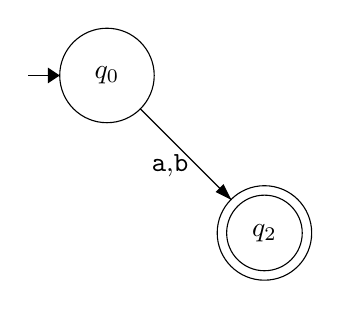
\begin{tikzpicture}[scale=0.2]
\tikzstyle{every node}+=[inner sep=0pt]
\draw [black] (-5,0) -- (-3,0);
\fill [black] (-3,0) -- (-3.75,-.5) -- (-3.75,.5);
\draw [black] (0,0) circle (3);
\draw (0,0) node {$q_0$};

\draw (4, -5) node [below] {{\tt a},{\tt b}};
\draw [black] (2.1,-2.1) -- (7.9,-7.9);
\fill [black] (7.9,-7.9) -- (6.9,-7.4) -- (7.4,-6.9);
\draw [black] (10,-10) circle (3);
\draw [black] (10,-10) circle (2.4);
\draw (10,-10) node {$q_2$};
\end{tikzpicture}

\end{figure}

В новому автоматі функція $\delta$ визначається лише для нетупикових станів.

\subsubsection{Еквівалентні стани}

Автомат, у котрого відсутні недосяжні та тупикові стани, піддається подальшій мінімізації шляхом ``склеювання'' еквівалентних станів. Продемонструємо це на конкретному прикладі:
\begin{figure}[H]
	\centering
	% cd ..\..\Users\NikitaSkybytskyi\Desktop\c3s1\complex-analysis
\documentclass[a4paper, 12pt]{article}
\usepackage[utf8]{inputenc}
\usepackage[english, ukrainian]{babel}

\usepackage{amsmath, amssymb}
\usepackage{multicol}
\usepackage{graphicx}
\usepackage{float}
\usepackage{multicol}

\usepackage{amsthm}
\newtheorem{theorem}{Теорема}[subsection]
\newtheorem*{theorem*}{Теорема}
\newtheorem{lemma}{Лема}[subsection]
\newtheorem*{lemma*}{Лема}
\newtheorem*{remark*}{Зауваження}
\theoremstyle{definition}
\newtheorem*{definition}{Визначення}
\newtheorem{problem}{Задача}[section]
\newtheorem*{solution}{Розв'язок}
\newtheorem{example}{Приклад}
\newtheorem*{example*}{Приклад}
\newtheorem*{hint}{Вказівка}

\newcommand{\Max}{\displaystyle\max\limits}
\newcommand{\Sum}{\displaystyle\sum\limits}
\newcommand{\Int}{\displaystyle\int\limits}
\newcommand{\Lim}{\displaystyle\lim\limits}

\newcommand{\RR}{\mathbb{R}}
\newcommand{\ZZ}{\mathbb{Z}}

\newcommand*\diff{\mathop{}\!\mathrm{d}}
\newcommand*\Diff[1]{\mathop{}\!\mathrm{d^#1}}

\DeclareMathOperator{\Real}{Re}
\DeclareMathOperator{\Imag}{Im}

\DeclareMathOperator{\Arg}{Arg}

\DeclareMathOperator{\Ln}{Ln}

\DeclareMathOperator{\Arctan}{Arctan}
\DeclareMathOperator{\Arcsin}{Arcsin}
\DeclareMathOperator{\Arccos}{Arccos}
\DeclareMathOperator{\Arccosh}{Arccosh}
\DeclareMathOperator{\Arctanh}{Arctanh}

\DeclareMathOperator{\arcsinh}{arcsinh}
\DeclareMathOperator{\arccosh}{arccosh}
\DeclareMathOperator{\arctanh}{arctanh}
\DeclareMathOperator{\arccoth}{arccoth}

\newcommand{\varLimsup}{\varlimsup\limits}

\makeatletter
\newcommand\xLeftrightarrow[2][]{%
  \ext@arrow 9999{\longLeftrightarrowfill@}{#1}{#2}}
\newcommand\longLeftrightarrowfill@{%
  \arrowfill@\Leftarrow\relbar\Rightarrow}
\makeatother

\renewcommand{\epsilon}{\varepsilon}
\renewcommand{\phi}{\varphi}

\allowdisplaybreaks
\setlength\parindent{0pt}
\numberwithin{equation}{subsection}

\usepackage{xcolor}
\usepackage{hyperref}
\hypersetup{unicode=true,colorlinks=true,linktoc=all,linkcolor=red}

\numberwithin{equation}{section}% reset equation counter for sections
\numberwithin{equation}{subsection}
% Omit `.0` in equation numbers for non-existent subsections.
\renewcommand*{\theequation}{%
  \ifnum\value{subsection}=0 %
    \thesection
  \else
    \thesubsection
  \fi
  .\arabic{equation}%
}


\title{{\Huge МАТЕМАТИЧНА ФІЗИКА}}
\author{Скибицький Нікіта}
\date{\today}

\usepackage{amsthm}
\usepackage[dvipsnames]{xcolor}
\usepackage{thmtools}
\usepackage[framemethod=TikZ]{mdframed}

\theoremstyle{definition}
\mdfdefinestyle{mdbluebox}{%
	roundcorner = 10pt,
	linewidth=1pt,
	skipabove=12pt,
	innerbottommargin=9pt,
	skipbelow=2pt,
	nobreak=true,
	linecolor=blue,
	backgroundcolor=TealBlue!5,
}
\declaretheoremstyle[
	headfont=\sffamily\bfseries\color{MidnightBlue},
	mdframed={style=mdbluebox},
	headpunct={\\[3pt]},
	postheadspace={0pt}
]{thmbluebox}

\mdfdefinestyle{mdredbox}{%
	linewidth=0.5pt,
	skipabove=12pt,
	frametitleaboveskip=5pt,
	frametitlebelowskip=0pt,
	skipbelow=2pt,
	frametitlefont=\bfseries,
	innertopmargin=4pt,
	innerbottommargin=8pt,
	nobreak=true,
	linecolor=RawSienna,
	backgroundcolor=Salmon!5,
}
\declaretheoremstyle[
	headfont=\bfseries\color{RawSienna},
	mdframed={style=mdredbox},
	headpunct={\\[3pt]},
	postheadspace={0pt},
]{thmredbox}

\declaretheorem[%
style=thmbluebox,name=Теорема,numberwithin=section]{theorem}
\declaretheorem[style=thmbluebox,name=Лема,sibling=theorem]{lemma}
\declaretheorem[style=thmbluebox,name=Твердження,sibling=theorem]{proposition}
\declaretheorem[style=thmbluebox,name=Наслідок,sibling=theorem]{corollary}
\declaretheorem[style=thmredbox,name=Приклад,sibling=theorem]{example}

\mdfdefinestyle{mdgreenbox}{%
	skipabove=8pt,
	linewidth=2pt,
	rightline=false,
	leftline=true,
	topline=false,
	bottomline=false,
	linecolor=ForestGreen,
	backgroundcolor=ForestGreen!5,
}
\declaretheoremstyle[
	headfont=\bfseries\sffamily\color{ForestGreen!70!black},
	bodyfont=\normalfont,
	spaceabove=2pt,
	spacebelow=1pt,
	mdframed={style=mdgreenbox},
	headpunct={ --- },
]{thmgreenbox}

\mdfdefinestyle{mdblackbox}{%
	skipabove=8pt,
	linewidth=3pt,
	rightline=false,
	leftline=true,
	topline=false,
	bottomline=false,
	linecolor=black,
	backgroundcolor=RedViolet!5!gray!5,
}
\declaretheoremstyle[
	headfont=\bfseries,
	bodyfont=\normalfont\small,
	spaceabove=0pt,
	spacebelow=0pt,
	mdframed={style=mdblackbox}
]{thmblackbox}

% \theoremstyle{theorem}
\declaretheorem[name=Запитання,sibling=theorem,style=thmblackbox]{ques}
\declaretheorem[name=Вправа,sibling=theorem,style=thmblackbox]{exercise}
\declaretheorem[name=Зауваження,sibling=theorem,style=thmgreenbox]{remark}

\theoremstyle{definition}
\newtheorem{claim}[theorem]{Твердження}
\newtheorem{definition}[theorem]{Визначення}
\newtheorem{fact}[theorem]{Факт}

\newtheorem{problem}{Задача}[section]
\renewcommand{\theproblem}{\thesection\Alph{problem}}
\newtheorem{sproblem}[problem]{Задача}
\newtheorem{dproblem}[problem]{Задача}
\renewcommand{\thesproblem}{\theproblem$^{\star}$}
\renewcommand{\thedproblem}{\theproblem$^{\dagger}$}
\newcommand{\listhack}{$\empty$\vspace{-2em}} 

\begin{document}
\tableofcontents

\setcounter{section}{2}

\section{Побудова математичних моделей базових фізичних процесів}

\setcounter{subsection}{-1}
\subsection{Оператор \texorpdfstring{$\nabla$}{nabla} (лікбез математичної теорії поля)}

\begin{definition}[оператора $\nabla$ в $\RR^2$]
    Для двовимірного евклідового простору $\RR^2$ у прямокутній декартовій системі координат \it{оператор набла} визначається наступним чином:
    \begin{equation}
    	\nabla = \frac{\partial}{\partial x} \vec{i} + \frac{\partial}{\partial y} \vec{j}
    \end{equation}
    де $\vec{i}$, $\vec{j}$ --- одиничні вектори по вісям $x$ і $y$ відповідно.
\end{definition}

\begin{definition}[оператора $\nabla$ в $\RR^3$]
    \begin{equation}
    	\nabla = \frac{\partial}{\partial x} \vec{i} + \frac{\partial}{\partial y} \vec{j} + \frac{\partial}{\partial z} \vec{k},
    \end{equation}
    де $\vec{i}$, $\vec{j}$, $\vec{k}$ --- одиничні вектори по вісям $x$, $y$ і $z$ відповідно.
\end{definition}

\subsubsection{Властивості оператора \texorpdfstring{$\nabla$}{nabla}}

\begin{definition}[градієнту через оператор $\nabla$]
	Якщо ``скалярно помножити'' вектор $\nabla$ на скалярну функцію $f = f(x, y, z)$, то вийде вектор:
	\begin{equation}
    	\nabla f = \frac{\partial f}{\partial x} \vec{i} + \frac{\partial f}{\partial y} \vec{j} + \frac{\partial f}{\partial z} \vec{k} = \left( \frac{\partial f}{\partial x}, \frac{\partial f}{\partial y}, \frac{\partial f}{\partial z} \right) = \grad f,
    \end{equation}
    який є нічим іншим як \it{градієнтом} $\grad f$ функції $f$.
\end{definition}

\begin{definition}[дивергенції через оператор $\nabla$]
	Якщо ``скалярно помножити'' вектор $\nabla$ на вектор-функцію
	\begin{equation}
	    \vec{F} = (f, g, h) = (f(x, y, z), g(x, y, z), h(x, y, z)),
	\end{equation}
	то вийде скаляр:
	\begin{equation}
    	\nabla \cdot \vec{F} = \frac{\partial f}{\partial x} + \frac{\partial g}{\partial y} + \frac{\partial h}{\partial z} = {\bf div} \vec{F},
    \end{equation}
    який є нічим іншим як \it{дивергенцією} $\divergence \vec{F}$ функції $\vec{F}$.
\end{definition}

\begin{definition}[ротора через оператор $\nabla$]
	Якщо ``векторно помножити'' вектор $\nabla$ на вектор-функцію
	\begin{equation}
	    \vec{F} = (f, g, h) = (f(x, y, z), g(x, y, z), h(x, y, z)),
	\end{equation}
	то вийде вектор:
	\begin{equation}
    	\begin{aligned}
        	\nabla \times \vec{F} &= \begin{vmatrix}
        		\vec{i} & \vec{j} & \vec{k} \\
        		\frac{\partial}{\partial x} & \frac{\partial}{\partial y} & \frac{\partial}{\partial z} \\
        		f & g & h
    		\end{vmatrix} = \\
    		&= \left( \frac{\partial h}{\partial y} - \frac{\partial g}{\partial z} \right) \vec{i} + \left( \frac{\partial f}{\partial z} - \frac{\partial h}{\partial x} \right) \vec{j} + \left( \frac{\partial g}{\partial x} - \frac{\partial f}{\partial y} \right) \vec{k} = \rot \vec{F}.
    	\end{aligned}
    \end{equation}
    який є нічим іншим як \it{ротором} $\rot \vec{F}$ функції $\vec{F}$.
\end{definition}

\begin{definition}[оператора Лапласа через оператор $\nabla$]
	Склаярний добуток $\nabla \cdot \nabla = \nabla^2$ є ніщо янше як оператор Лапласа, який також позначається $\Delta$. \medskip

	У декартових координатах оператор Лапласа має вигляд
	\begin{equation}
    	\Delta = \frac{\partial^2}{\partial x^2} + \frac{\partial^2}{\partial y^2} + \frac{\partial^2}{\partial z^2}.
    \end{equation}
\end{definition}

\subsubsection{Оператори другого порядку}

Оскільки існують різні способи множення веткорів і скалярів, з допомогою оператор набла можна записати різі види ``диференціювання''. так, комбінування склаярних і векторних добутків дає 7 різних варіантів ``похідних'' другого порядку:

\begin{align}
	& \divergence (\grad f) = \nabla \cdot (\nabla f) \\
	& \rot (\grad f) = \nabla \times (\nabla f) \\
	& \Delta f = \nabla^2 f) \\
	& \grad (\divergence \vec{F}) = \nabla (\nabla \cdot \vec{F}) \\
	& \divergence (\rot \vec{F}) = \nabla \cdot (\nabla \times \vec{F}) \\
	& \rot (\rot \vec{F}) = \nabla \times (\nabla \times \vec{F}) \\
	& \Delta \vec{F} = \nabla^2 \vec{F}
\end{align}

Для достатньо гладких полів (двічі неперервно диференційовних) ці оператори не незалежні. Два з них тотожньо дорівнюють нулю:

\begin{gather}
	\rot (\grad f) = \nabla \times (\nabla f) = (\nabla \times \nabla) f = 0 \\
	\divergence (\rot \vec{F}) = \nabla \cdot (\nabla \times \vec{F}) = (\nabla \times \nabla) \cdot \vec{F} = 0.
\end{gather}

Два завжди рівні:

\begin{equation}
	\divergence (\grad f) = \nabla \cdot (\nabla f) = (\nabla \cdot \nabla) f = \nabla^2 f = \Delta f.
\end{equation}

А решта три пов'язані співвідношенням:

\begin{equation}
	\nabla \times (\nabla \vec {F})= \nabla (\nabla \cdot \vec{F}) - \nabla^2 \vec{F}.
\end{equation}

І ще один може бути виражене через тензорний добуток векторів:

\begin{equation}
	\nabla (\nabla \cdot \vec{F}) = \nabla \cdot (\nabla \otimes \vec {F})
\end{equation}

\subsubsection{Приклади}

\begin{example}
	Нехай $z = z(x, y) = x y$, тоді
	\begin{equation}
		\nabla z = \frac{\partial z}{\partial x} \vec{i} + \frac{\partial z}{\partial y} \vec{j} = y \vec{i} + x \vec{j}.
	\end{equation}
\end{example}

\begin{example}
	Нехай $z = z(x, y) = 30 y x^3$, тоді
	\begin{equation}
		\nabla z = \frac{\partial z}{\partial x} \vec{i} + \frac{\partial z}{\partial y} \vec{j} = 90 y x^2 \vec{i} + 30 x^3 \vec{j}.
	\end{equation}
\end{example}

\subsection{Математичні моделі розповсюдження тепла та дифузії речовини}

Для запису математичної моделі введемо величини:
\begin{itemize}
	\item $x = (x_1, x_2, x_3) \in G \subset \RR^3$ об'єм тіла, $t$ --- час;
	\item $u(x, t)$ --- температура в точці $x$ у момент часу $t$;
	\item $c(x)$ --- теплоємність (кількість тепла, яка необхідна, для підняти температуру одиниці маси тіла на один градус);
	\item $k(x)$ --- теплопровідність речовини (здатність проводити тепло);
	\item $\rho(x)$ --- щільність речовини;
	\item $f(x, t)$ --- інтенсивність джерел теплової енергії в точці $x$ в момент часу $t$.
\end{itemize}

\subsubsection{Закон збереження теплової енергії}

Складемо баланс теплової енергії для довільного об'єму тіла $G$ за довільний інтервал часу $t_1 < t < t_2$. Для цього обчислимо кількість тепла, яка міститься в нескінченно малому об'ємі $\diff G$: 
\begin{equation}
	\rho(x) \cdot \diff G \cdot c(x) \cdot u(x, t)
\end{equation}
та в об'ємі $G$ в момент часу $t$:
\begin{equation}
	Q_1(t) = \Iiint_G c(x) \rho(x) u(x, t) \diff G.
\end{equation}

Припустимо, що з часом температура змінилася від значення $u(x, t_1)$ до значення $u(x, t_2)$. Обчислимо кількість тепла, витрачену на зміну температури:
\begin{equation}
	\Delta Q_1(t_1, t_2) = Q_1(t_2) - Q_1(t_1) = \Iiint_G c(x) \rho(x) (u(x, t_2) - u(x, t_1)) \diff G.
\end{equation}

Температура в об'ємі $G$ може змінюватись за рахунок таких факторів:
\begin{enumerate}
	\item нерівномірності нагрівання тіла, викликає потік тепла через поверхню $S$, яка обмежує уявне тіло об'єму $G$;
	\item зміна кількості тепла за рахунок внутрішніх теплових джерел.
\end{enumerate}

Нехай $\vec n$ --- зовнішня нормаль до поверхні $S$. Обчислимо кількість тепла, яка поступає всередину об'єму $G$ через елементарну поверхню $\diff S$ в одиницю часу: 
\begin{equation}
	\diff Q(x, t) = k(x) \cdot \frac{\partial u(x, t)}{\partial \vec n} \cdot \diff S
\end{equation}

Ця формула є математичним виразом фізичного закону Фур'є. \medskip

Кількість тепла, яка проходить через всю поверхню $S$ за час від $t_1$ до $t_2$ обчислюється за формулою
\begin{equation}
	Q_2(t_1, t_2) = \Int_{t_1}^{t_2} \Iint_S \left( k(x) \cdot \frac{\partial u(x, t)}{\partial \vec n} \right) \diff S \diff t.
\end{equation}

Кількість тепла за рахунок теплових джерел в об'ємі $G$ можна обчислити у вигляді:
\begin{equation}
	Q_3(t_1, t_2) = \Int_{t_1}^{t_2} \Iiint_G f(x, t) \diff G \diff t.
\end{equation}

Таким чином можна записати 
\begin{law*}[збереження теплової енергії]
	Виконується співвідношення:
	\begin{equation}
		\Delta Q_1(t_1, t_2) = Q_2(t_1, t_2) + Q_3(t_1, t_2),
	\end{equation}
\end{law*}
або після підстановки усіх величин маємо 
\begin{law*}[збереження теплової енергії  в інтегральному вигляді]
	Виконується співвідношення:
	\begin{multline}
		\Iiint_G c(x) \rho(x) (u(x, t_2) - u(x, t_1)) \diff G = \\
		= \Int_{t_1}^{t_2} \Iint_S \left( k(x) \cdot \frac{\partial u(x, t)}{\partial \vec n} \right) \diff S \diff t + \Int_{t_1}^{t_2} \Iiint_G f(x, t) \diff G \diff t.
	\end{multline}
\end{law*}

Для перетворення першого інтегралу правої частини останньої рівності застосуємо формулу Остроградського Гауса, 
\begin{equation}
	\Iint_S \langle A, \vec n \rangle \diff S = \Iiint_G \Big(\nabla \cdot \vec A\Big) \diff G,
\end{equation}
де $\vec A$ --- векторне поле,
\begin{equation}
	\nabla \cdot A = \frac{\partial A_1}{\partial x_1} + \frac{\partial A_2}{\partial x_2} + \frac{\partial A_3}{\partial x_3}.
\end{equation}

В результаті отримаємо:
\begin{multline}
	\Int_{t_1}^{t_2} \Iiint_G \left( c(x)\rho(x) \frac{\partial u(x, t)}{\partial t} \right) \diff G \diff t = \\
	= \Int_{t_1}^{t_2} \Iiint_G \left( \nabla \cdot (k(x) \nabla u) \right) \diff G \diff t + \Int_{t_1}^{t_2} \Iiint_G f(x, t) \diff G \diff t.
\end{multline}

Враховуючи, що остання рівність отримана для довільного об'єму $G$ та довільних моментів часу, можна зробити висновок, що вона має місце тоді і лише тоді, коли має місце рівність підінтегральних виразів:
\begin{equation}
	\label{eq:thermal-energy-is-const}
	c(x) \rho(x) \frac{\partial u(x, t)}{\partial t} =\nabla\cdot (k(x) \nabla u) + f(x, t),
\end{equation}
де $x \in G$, $t > 0$. \medskip

Це рівняння повинно виконуватись для кожної точки $x$ реального фізичного об'єму тіла (збережемо для нього позначення $G$, а для його поверхні позначення $S$), та для кожного моменту часу $t$. \medskip

Для виділення єдиного розв'язку цього рівняння окрім самого диференціального рівняння необхідно задавати додаткові умови на границі просторово-часової області. Будемо використовувати фізичні міркування для задавання таких умов.

\begin{enumerate}
	\item Якщо на границі області відома температура тіла, тоді на границі тіла задають умову Діріхле.

	\begin{definition}[умови Діріхле]
		Крайовою умовою першого роду, або \it{умовою Діріхле} називають співвідношення
		\begin{equation}
			\left. u(x, t) \right|_{x \in S} = v(x, t).		 							
		\end{equation}
	\end{definition}

	\item Якщо на границі області відомий тепловий потік в одиницю часу, який поступає всередину тіла через одиничну площу, тоді на границі задають граничну умову Неймана.

	\begin{definition}[умови Неймана]
		Крайовою умовою другого роду, або \it{умовою Неймана} називають співвідношення
		\begin{equation}
			\left. k(x) \frac{\partial u(x, t)}{\partial \vec n} \right|_{x \in S} = q(x, t).
		\end{equation}
	\end{definition}

	\item Якщо на границі тіла відбувається конвективний теплообмін з оточуючим середовищем відомої температури згідно до закону Ньютона, тоді на границі задають крайову умову Ньютона
	\begin{definition}[умови Ньютона]
		Крайовою умовою третього роду, або \it{умовою Ньютона} називають співвідношення
		\begin{equation}
			\left. k(x) \frac{\partial u(x, t)}{\partial \vec n} \right|_{x \in S} = \left. \alpha(x, t) (v(x, t) - u(x, t)) \right|_{x \in S},
		\end{equation}
		де $\alpha(x, t) > 0$ --- коефіцієнт теплообміну, $v(x, t)$ --- температура оточуючого середовища.
	\end{definition}

	\item В початковий момент часу задають температура усіх внутрішніх точок тіла:
	\begin{equation}
		\left. u(x, t) \right|_{t = 0} = u_0(x).
	\end{equation}

	\begin{definition}[початкової умови]
		\it{Початковою умовою} називається співвідношення
		\begin{equation}
			\left. u(x, t) \right|_{t = 0} = u_0(x),
		\end{equation}
		при цьому $u_0(x)$ називається \it{початковою температурою}.
	\end{definition}
\end{enumerate}

\subsubsection{Частинні випадки рівняння теплопровідності}

\begin{remark}
	У випадку, коли коефіцієнт теплопровідності та інтенсивність теплових джерел залежить не лише від точки простору і часу, а і від самої температури, тобто $k = k(u, x, t)$, $f = f(u, x, t)$, лінійне диференціальне рівняння \eqref{eq:thermal-energy-is-const} стає квазілінійним, тобто лінійним відносно старших похідних.
\end{remark}

Окрім загального вигляду рівняння теплопровідності, у практичних випадках часто використовуються частинні випадки рівняння. \medskip

Зокрема, можна розглядати розповсюдження тепла в одновимірних та двовимірних тілах:
\begin{itemize}
	\item У пластині:
	\begin{equation}
		\nabla \cdot (k(x) \nabla u(x, t)) = \frac{\partial}{\partial x_1} \left( k(x) \frac{\partial u(x, t)}{\partial x_1} \right) + \frac{\partial}{\partial x_2} \left( k(x) \frac{\partial u(x, t)}{\partial x_2} \right).
	\end{equation}
	\item У стрижні:
	\begin{equation}
		\nabla \cdot (k(x) \nabla u(x, t)) = \frac{\partial}{\partial x} \left( k(x) \frac{\partial u(x, t)}{\partial x} \right).
	\end{equation}
\end{itemize}

Для однорідних тіл усі коефіцієнти рівняння можна вважати константами, зокрема $c = c_0$, $\rho = \rho_0$, $k = k_0$. В результаті вищезгадане диференціальне рівняння буде мати вигляд
\begin{equation}
	\frac{\partial u(x, t)}{\partial t} = a^2 \Delta u + \frac{1}{c_0 \rho_0} \cdot f(x, t),
\end{equation}
де 
\begin{equation}
	a^2 = \frac{k_0}{c_0 \rho_0} > 0,
\end{equation}
і було введено
\begin{definition}[оператор Лапласа]
	\it{Оператором Лапласа} називається диференціальний оператор $\Delta$ що діє на функцію $u(x, t)$ по векторній змінній $x$ наступним чином:
	\begin{equation}
		\Delta u(x, t) = \nabla \cdot (\nabla u(x, t)) = \Sum_{i = 1}^n \frac{\partial^2 u(x, t)}{\partial x_i^2}.
	\end{equation}
\end{definition}

\begin{remark}
	Зокрема одновимірне рівняння теплопровідності має вигляд:
	\begin{equation}
		\frac{\partial u(x, t)}{\partial t} = a^2 \frac{\partial^2 u(x, t)}{\partial x^2} + \frac{1}{c_0 \rho_0} f(x, t).
	\end{equation}
\end{remark}

\subsubsection{Рівняння дифузії речовини}

Процес дифузії речовини це процес вирівнювання концентрації речовини у розчинах, розплавах або в сумішах. Фізика вирівнювання температури в тілах та концентрації у розчинах чи розплавах має багато схожих рис і з цього приводу навіть процес розповсюдження тепла називають дифузією тепла. \medskip

Для отримання моделі дифузії речовини використаємо наступну таблицю аналогії.
\begin{table}[H]
	\centering
	\begin{tabular}{| C{3.75cm} | C{3.75cm} | L{4.5cm} |}
		\hline
		Дифузія & Теплопровідність & Пояснення \\ \hline
		$u(x, t)$ & $u(x, t)$ & Концентрація речовини в розчині, або у розплаві \\ \hline
		$c(x)$ & $c(x) \rho(x)$ & Коефіцієнт пористості, відображає відношення об'єму пор до загального об'єму тіла і вказує на кількість речовини необхідну для зміни концентрації на одну одиницю в одиниці об'єму. \\ \hline
	\end{tabular}
\end{table}

\begin{table}[H]
	\centering
	\begin{tabular}{| C{3.75cm} | C{3.75cm} | L{4.5cm} |}
		\hline
		Дифузія & Теплопровідність & Пояснення \\ \hline
		$D \dfrac{\partial u}{\partial \vec n} \diff S$ & $k \dfrac{\partial u}{\partial \vec n} \diff S$ & Закон Нерста, описує кількість речовини, яка поступає всередину тіла через його поверхню в одиницю часу за рахунок нерівномірності концентрації. \\ \hline
		$f(x, t)$ & $f(x, t)$ & Інтенсивність джерела речовини в середині об'єму. \\ \hline
 		$D \dfrac{\partial u}{\partial \vec n} = \alpha \left. (v - u)\right|_S$ & $k \dfrac{\partial u}{\partial \vec n} = \alpha \left. (v - u)\right|_S$ & Кількість речовини, яка поступає через поверхню $S$ тіла за законом, аналогічним закону Ньютона,
 		$v$ --- відома концентрація речовини в тому чи іншому середовищі; $\alpha$ --- коефіцієнт проникності поверхні. \\ \hline
 	\end{tabular}
\end{table}

Побудови математичної моделі процесу дифузії відбувається за аналогією згідно до попередньої таблиці. \medskip

Кількість речовини, яка витрачена для зміни концентрації від $u(x, t_1) \to u(x, t_2)$, $t_1 < t_2$ має вигляд:
\begin{equation}
	\Delta Q_1(t_1, t_2) = Q_1(t_2) - Q_1(t_1) = \Iiint_G c(x) (u(x, t_2) - u(x, t_1)) \diff G.
\end{equation}

Кількість речовини, яка проходить через всю поверхню $S$ за час від $t_1 \to t_2$:
\begin{equation}
	Q_2(t_1, t_2) = \Int_{t_1}^{t_2} \Iint_S \left( D(x, t) \frac{\partial u}{\partial \vec n} \right) \diff S \diff t.
\end{equation}

Кількість речовини, яка поступає за рахунок джерел речовини в об'ємі $G$ за час від $t_1$ до $t_2$:
\begin{equation}
	Q_3(t_1, t_2) = \Int_{t_1}^{t_2} \Iiint_G f(x, t) \diff G \diff t.
\end{equation}

Отже, отримали 
\begin{law*}[збереження маси]
	Вионується співвідношення:
	\begin{equation}
		\Delta Q_1(t_1, t_2) = Q_2(t_1, t_2) + Q_3(t_1, t_2).
	\end{equation}
\end{law*}
а також
\begin{law*}[збереження маси в інтегральному вигляді]
	Вионується співвідношення:
	\begin{multline}
		\Iiint_G c(x) (u(x, t_2) - u(x, t_1)) \diff G = \\
		= \Int_{t_1}^{t_2} \Iint_S \left( D(x, t) \frac{\partial u(x, t)}{\partial \vec n} \right) \diff S \diff t + \Int_{t_1}^{t_2} \Iiint_G f(x, t) \diff G \diff t.
	\end{multline}
\end{law*}

Після застосування формули Остроградського-Гауса та прирівнювання підінтегральних виразів отримаємо рівняння дифузії речовини у вигляді:
\begin{equation}
	c(x) \frac{\partial u}{\partial t} = \nabla \cdot (D(x, t) \nabla u) + f(x, t),
\end{equation}
де $x \in G$, $t > 0$. \medskip

Додаткові умови на границі області задають аналогічно умовам для рівняння теплопровідності:
\begin{enumerate}
	\item Якщо відома концентрація речовини на поверхні:
	\begin{equation}
		\left. u(x, t) \right|_{x \in S} = v(x, t);
	\end{equation}

	\item Якщо на границі відомий потік речовини:
	\begin{equation}
		\left. D \cdot \frac{\partial u(x, t)}{\partial \vec n} \right|_{x \in S} = g(x, t);
	\end{equation}

	\item Якщо на границі відбувається обмін речовиною з оточуючим середовищем через напівпроникливу мембрану за законом аналогічним закону Ньютона:
	\begin{equation}
		\left. D(x,t) \frac{\partial u(x, t)}{\partial \vec n} \right|_{x \in S} = \alpha(x,t) \left. ( v(x, t) - u(x, t) ) \right|_{x \in S};
	\end{equation}

	\item Якщо в початковий момент часу відома концентрація речовини:
	\begin{equation}
		u(x, 0) = u_0(x).
	\end{equation}
\end{enumerate}

\begin{remark}
	У випадку, коли коефіцієнти рівняння та граничних умов не залежать від часу $t$, розв'язок рівняння не залежить від часу в результаті отримаємо стаціонарне рівняння теплопровідності та дифузії:
	\begin{align}
		\nabla \cdot (k(x) \nabla u(x)) &= -f(x), \\
		\nabla \cdot (D(x) \nabla u(x)) &= -f(x).
	\end{align}
\end{remark}

\subsubsection{Задача Стефана (задача про остигання та затвердіння розплавленого металу)}

Вертикальний циліндричний посуд заповнений розплавленим металом, який знаходиться при заданій температурі $U_0 > U_{melt}$ - температура плавління металу. Починаючи з моменту часу $t_0$ вільна поверхня розплавленого металу підтримується при постійній температурі $U_1 < U_{melt}$. Поставимо задачу про остудження та затвердіння металу, якщо дно і бокова поверхня посуду теплоізольовані. Термічними деформаціями об'єму будемо нехтувати тобто процес розповсюдження тепла відбувається лише вздовж вісі циліндру. Введемо позначення: 
\begin{itemize}
 	\item $\rho_s$, $\rho_l$ --- щільність твердої (eng. \it{solid}) та рідкої (eng. \it{liquid}) фази металу;
	\item $c_s$, $c_l$ --- теплоємність твердої та рідкої фази металу;
	\item $k_s$, $k_l$ --- теплопровідність твердої та рідкої фази металу;
	\item $\xi(t)$ --- положення границі розділу твердої та рідкої фаз;
	\item $L$ --- висота циліндру, $S$ --- площа основи циліндру; 
	\item $\lambda$ --- питома теплота плавлення;
	\item $u(x, t)$ --- температура в момент часу $t$ в точці $x$.
\end{itemize}

Деякі з введених позначень краще видно на наступній ілюстрації:
\begin{figure}[H]
	\centering
	\includegraphics[width=.7\textwidth]{{../img/7-1}.mps}
\end{figure}

Отримаємо рівняння теплового балансу для нескінченно малого об'єму розплавленого металу, який знаходиться між перерізами $x$ та $x + \Delta x$ за проміжок часу від $t$ до $t + \Delta t$. \medskip

Обчислимо кількість тепла, яка необхідна для зміни температури у виділеному елементарному об'ємі від значення $u(x, t)$ до значення $u(x, t + \Delta t)$. Кількість тепла, що міститься в виділеному об'ємі в момент часу $t$ можна обчислити за формулою
\begin{equation}
	\diff Q(t) = c_l \cdot \rho_l \cdot S \cdot \Delta x \cdot u(x, t).
\end{equation}

Аналогічно для моменту часу $t + \Delta t$ кількість тепла дорівнює
\begin{equation}
	\diff Q(t + \Delta t) = c_l \cdot \rho_l \cdot S \cdot \Delta x \cdot u(x, t + \Delta t).
\end{equation}

При цьому нехтуємо, зміною температури по просторовій змінній у середині елементарного об'єму. Тоді кількість тепла, необхідна для зміни температури всередині об'єму дорівнює:
\begin{equation}
	\Delta Q(t, t + \Delta t) = c_l \cdot \rho_l \cdot S \cdot \Delta x \cdot (u(x, t + \Delta t) - u(x, t)).
\end{equation}

Ця зміна може відбуватися за рахунок теплових потоків, через перерізи $x$ та $x + \Delta x$. Підрахуємо кількість тепла, яка поступає всередину тіла через переріз $x + \Delta x$ за час $\Delta t$:
\begin{equation}
	\diff Q(x + \Delta x) = k_l \frac{\partial u(x + \Delta x, t)}{\partial \vec n} S \Delta t= k_l \frac{\partial u(x + \Delta x, t)}{\partial x} S \Delta t
\end{equation} 
 
Напрям нормалі $\vec n$ в цьому перерізі співпадає з напрямом вісі $Ox$. \medskip

Кількість тепла, яка поступає всередину тіла через переріз $x$ за час $\Delta t$ можна записати у вигляді:
\begin{equation}
	\diff Q(x) = k_l \frac{\partial u(x, t)}{\partial \vec n} S \Delta t = - k_l \frac{\partial u(x, t)}{\partial x} S \Delta t
\end{equation} 

Таким чином можна скласти рівняння теплового балансу:
\begin{equation}
	\diff Q(t, t + \Delta t) = \diff Q(x + \Delta x) + \diff Q(x).
\end{equation}
 
Або після підстановки відповідних значень поділених на $\Delta x \cdot \Delta t \cdot S$ отримаємо:
\begin{equation}
	\frac{c_l \rho_l (u(x, t + \Delta t) - u(x, t))}{\Delta t} = k_l \left( \frac{\partial u(x + \Delta x, t)}{\partial x} - \frac{\partial u(x, t)}{\partial x} \right) \frac{1}{\Delta x}.
\end{equation}
 
Після граничного переходу коли $\Delta x$ та $\Delta t$ прямують до нуля, отримаємо диференціальне рівняння:
\begin{equation}
	\label{eq:liquid-phase-diff-eq}
	c_l \rho_l \frac{\partial u(x, t)}{\partial t} = k_l \frac{\partial^2 u(x, t)}{\partial x^2},
\end{equation}
де $\xi(t) < x < L$, $t > t_0$. \medskip

Аналогічні міркування дозволяють отримати рівняння для твердої фази:
\begin{equation}
	\label{eq:solid-phase-diff-eq}
	c_s \rho_s \frac{\partial u(x, t)}{\partial t} = k_s \frac{\partial^2 u(x, t)}{\partial x^2},
\end{equation}
де $0 < x < \xi(t)$, $t > t_0$. \medskip

\begin{definition}[співвідношення на границі розділу фаз]
	Температура при переході через границю розділу фаз повинна змінюватись неперервно і співпадати з температурою плавлення металу, тобто повинно виконуватись настуну співвідношення:
	\begin{equation}
		\label{eq:phase-border-conditions}
		u(\xi(t) - 0, t) = u(\xi(t) + 0, t) = U_{melt},
	\end{equation}
	яке називається \it{співвідношенням на границі розділу фаз}.
\end{definition}

Отримаємо рівняння теплового балансу для елементарного об'єму обмеженого перерізами $\xi(t) - \Delta x$ та $\xi(t) + \Delta x$. \medskip

За час $\Delta t$ затвердіє об'єм металу рівний
\begin{equation}
	(\xi(t + \Delta t) - \xi(t)) \cdot S.
\end{equation}

При цьому буде виділено кількість тепла рівна
\begin{equation}
	\diff Q_{melt} = (\xi(t + \Delta t) - \xi(t)) \cdot S \cdot \lambda \cdot \rho_s.
\end{equation}

Кількість тепла, яка надійде всередину об'єму за рахунок теплових потоків через відповідні перерізи за час $\Delta t$ може бути записана у вигляді:
\begin{equation}
	\Delta t \cdot S \cdot \left( k_l \cdot \frac{\partial u(\xi(t) + \Delta x, t)}{\partial x} - k_s \cdot \frac{\partial u(\xi(t) - \Delta x, t)}{\partial x}\right).
\end{equation}
 
Оскільки фазовий перехід відбувається при постійній температурі, то в околі границі розділу фаз $\xi(t)$ зміною температури по змінній $t$ можна нехтувати, в зв'язку з чим можна не враховувати кількість тепла, яка витрачається на зміну температури у виділеному елементарному об'ємі. \medskip

Рівняння теплового балансу для елементарного об'єму обмеженого перерізами $\xi(t) - \Delta x$ та $\xi(t) + \Delta x$ можна записати у вигляді:
\begin{multline}
	(\xi(t + \Delta t) - \xi(t)) S \lambda \rho_s = \\
	= \Delta t S \left( k_l \frac{\partial u(\xi(t) + \Delta x, t)}{\partial x} - k_s \frac{\partial u(\xi(t) - \Delta x, t)}{\partial x}\right)
\end{multline}

Поділивши обидві частини на $\Delta t$, скоротивши на $S$ і спрямувавши $\Delta x$, $\Delta t$ до нуля отримаємо співвідношення:
\begin{equation}
	\lambda \rho_s \frac{\partial \xi(t)}{\partial t} = k_l \frac{\partial u(\xi(t) + 0, t)}{\partial x} - k_s \frac{\partial u(\xi(t) - 0, t)}{\partial x}.
\end{equation}

\begin{definition}[внутрішніх граничних умов (умов спряження)]
	Останню умову 
	\begin{equation}
		\label{eq:conjugate-conditions}
		\lambda \rho_s \frac{\partial \xi(t)}{\partial t} = k_l \frac{\partial u(\xi(t) + 0, t)}{\partial x} - k_s \frac{\partial u(\xi(t) - 0, t)}{\partial x}.
	\end{equation}
	разом із співвідношенням \eqref{eq:phase-border-conditions} на границі розділу фаз називають \it{внутрішніми граничними умовами}, або \it{умовами спряження}.
\end{definition}

Запишемо початкові умови та умови на верхній та нижній основі циліндру:
\begin{itemize}
	\item В початковий момент часу задана температура розплавленого металу:
	\begin{equation}
		\label{eq:start-time-temp}
		u(x, t_0) = U_0, \quad 0 < x < L.
	\end{equation}
	
	\item На верхній основі задана температура:
	\begin{equation}
		\label{eq:upper-cylinder-border-temp}
		u(0, t) = U_1, \quad t > t_0.
	\end{equation}

	\item Нижня основа теплоізольована, тобто тепловий потік, який поступає всередину тіла дорівнює нулю:
	\begin{equation}
		\label{eq:lower-cylinder-border-temp-flow}
		\frac{\partial u(L, t)}{\partial x} = 0, \quad t > t_0.
	\end{equation}
	
	\item В початковий момент часу положення границі фазового переходу співпадає з верхньою основою циліндру: 
	\begin{equation}
		\label{eq:start-time-xi}
		\xi(t_0) = 0.
	\end{equation}
\end{itemize}

Таким чином, до моменту часу, коли весь метал затвердіє постановка задачі Стефана включає в себе диференційні рівняння \eqref{eq:liquid-phase-diff-eq}, \eqref{eq:solid-phase-diff-eq}, співвідношення на границі розділу фаз \eqref{eq:phase-border-conditions}, умови спряження \eqref{eq:conjugate-conditions}, початкові умови \eqref{eq:start-time-temp}, \eqref{eq:start-time-xi} та граничні умови \eqref{eq:upper-cylinder-border-temp}, \eqref{eq:lower-cylinder-border-temp-flow}. \medskip

\begin{remark}
	Після повного затвердіння металу, тобто коли $\xi(t_1) = L$, процес буде описуватись звичайним рівнянням теплообміну для $t > t_1$ з граничними умовами
	\begin{align}
		u(0, t) &= U_1, \\
		\frac{\partial u(L, t)}{\partial x} &= 0,
	\end{align}
	та початковою температурою $u(x, t_1)$.
\end{remark}

\end{document}

\end{figure}

Очевидно, що для наведеного вище скінченого автомата можна побудувати еквівалентний йому скінчений автомат з меншою кількістю станів:
\begin{figure}[H]
	\centering
	\section*{Заняття 8: Інтегрувальний множник. Випадки знаходження інтегрувального множника}

\subsection*{Аудиторні задачі}

Розв'язати диференціальні рівняння методом інтегрувального множника, знаючи, що вони мають вигляд $\mu = f(x)$ або $\mu = f(y)$:

\begin{problem}
	$(2 y + x y^3) \cdot \diff x + (x + x^2 y^2) \cdot \diff y = 0$.
\end{problem}

\begin{problem}
	$y^2 \cdot (x - 3 y) \cdot \diff x + (1 - 3 x y^2) \cdot \diff y = 0$.
\end{problem}

\begin{problem}
	$2 y \cdot \diff x + (y^2 - 6 x) \cdot \diff y = 0$.
\end{problem}

Зінтегрувати рівняння за допомогою множників $\mu(x + y)$, $\mu(x y)$, або $\mu(x - y)$

\begin{problem}
	$(y - a y / x + x) \cdot \diff x + a \cdot \diff y = 0$.
\end{problem}

\begin{problem}
	$y^2 \cdot \diff x + (x y - 1) \cdot \diff y = 0$.
\end{problem}

\subsection*{Домашнє завдання}

Розв'язати диференціальні рівняння методом інтегрувального множника, знаючи, що вони мають вигляд $\mu = f(x)$ або $\mu = f(y)$:

\begin{problem}
	$(1 + x^2 y) \cdot \diff x + x^2 \cdot (x + y) \cdot \diff y = 0$.
\end{problem}

\begin{problem}
	$(2 x y + a x) \cdot \diff x + \diff y = 0$.
\end{problem}

\begin{problem}
	$\diff x + (x + e^{-y} \cdot y^2) \cdot \diff y = 0$.
\end{problem}

Зінтегрувати рівняння за допомогою множників $\mu(x + y)$, $\mu(x y)$, або $\mu(x - y)$

\begin{problem}
	$\diff x + x \cdot \cot (x + y) \cdot (\diff x + \diff y) = 0$.
\end{problem}

\begin{problem}
	$(2 x^2 y + x) \cdot \diff y + (y + 2 x y^2 - x^2 y^3) \cdot \diff x = 0$.
\end{problem}

\end{figure}

Ми досягли бажаного нам результату шляхом ``склеювання'' двох станів $q_1 \equiv q_3$ та $q_2 \equiv q_4$. \medskip

Два стани $q_1$ та $q_2$ скінченого автомата $M$ називаються \textit{еквівалентними} (позначається $q_1 \equiv q_2$), якщо множини слів, які розпізнає автомат, починаючи з $q_1$ та $q_2$, співпадають. \medskip

Нехай $q_1$ та $q_2$ --- два різні стани скінченого автомата $M$, а $x \in \Sigma^\star$. Будемо говорити, що ланцюжок $x$ \textit{розрізняє} стани $q_1$ та $q_2$, якщо $(q_1,x) \models^\star (q_3, \varepsilon)$ та $(q_2,x) \models^\star (q_4, \varepsilon)$, причому рівно один зі станів $q_3$ і $q_4$ (не) належить множині заключних станів. \medskip

Стани $q_1$ та $q_2$ називаються \textit{$k$-нерозрізнені}, якщо не існує ланцюжка $x$ $(\left|x\right| \le k)$, що розрізняє стани $q_1$ та $q_2$. \medskip

Два стани $q_1$ та $q_2$ \textit{нерозрізнені}, якщо вони $k$-нерозрізнені для довільного $k$. \medskip

\textbf{Теорема.} \textit{Два стани $q_1$ та $q_2$ довільного скінченого автомата $M$ з $n$ станами нерозрізнені, якщо вони $(n - 2)$-нерозрізнені.} \medskip

\textbf{Доведення:} На першому кроці розіб'ємо множину станів скінченого автомата на дві підмножини: $F$ та $Q \setminus F$. На цій основі побудуємо відношення $\equiv^0$: $q_1 \equiv^0 q_2$, якщо обидва стани одночасно належать $F$ або $Q \setminus F$. \medskip

Побудуємо відношення $\equiv^k$: $q_1 \equiv^k q_2$, якщо $q_1 \equiv^{k - 1} q_2$ та $\delta(q_1,a) \equiv^{k - 1} \delta(q_2, a)$ для всіх $a \in \Sigma$. \medskip

Очевидно, кожна побудована множина містить не більше $(n-1)$ елементи. \medskip

Таким чином, можна отримати не більше $(n-2)$ уточнення відношення $\equiv^0$. \medskip

Відношення $\equiv^{n - 2}$ визначає класи еквівалентних станів автомата $M$.

\subsubsection{Алгоритм}

\textbf{Алгоритм [побудови мінімального скінченого автомата].}
\begin{enumerate}
	\item Побудувати скінчений автомат без тупикових станів.
	\item Побудувати скінчений автомат без недосяжних станів.
	\item Знайти множини еквівалентних станів та побудувати найменший (мінімальний) автомат.
\end{enumerate}

\subsection{Контрольні запитання}

\begin{enumerate}
	\item Які автомати називаються еквівалентними? % ті які задають одну мову
	\item Який стан автомату називається недосяжним? % той у який немає шляху з $q_0$ на діаграмі переходів
	\item Опишіть алгоритм пошуку недосяжних станів і доведіть його збіжність. \smallskip
	
	Бонус: оцініть складність цього алгоритму за часом і пам'\-ят\-тю.
	\item Який стан автомату називається тупиковим? % той з якого немає шляху в $F$ на діаграмі переходів
	\item Опишіть алгоритм пошуку тупикових станів і доведіть його збіжність. \smallskip
	
	Бонус: оцініть складність цього алгоритму за часом і пам'\-ят\-тю.
	\item Які стани називаються еквівалентними? % для яких не існує розрізняючого слова
	\item Опишіть алгоритм пошуку еквівалентних станів і доведіть його збіжність. \smallskip
	
	Бонус: оцініть складність цього алгоритму за часом і пам'яттю.
	\item Опишіть алгоритм мінімізації детермінованого скінченного автомату. \smallskip
	
	Бонус: виведіть з попередніх оцінок складність цього алгоритму за часом і пам'яттю.
\end{enumerate}
